% !TEX encoding = UTF-8 Unicode

\documentclass[10pt]{article}
\usepackage[margin=1.2in]{geometry}

%\usepackage{algpseudocode}
%\usepackage{algorithm}

\usepackage{graphicx}
\usepackage{fmtcount}

\usepackage{multirow}

\usepackage[hyphens]{url}
\usepackage{hyperref}

\usepackage{array}
\usepackage{amsmath}
\usepackage{amssymb}

%\usepackage{natbib}

\usepackage{mathtools}

\usepackage{listings}
\usepackage{color}
\usepackage{booktabs}

% keywords: fixme

\sloppy

\begin{document}

\title{{\tt C++11} ve {\tt x86-64} mimarisi kullanan efektif ters bit s{\i}ralamalar{\i}}

\author{Christian Knauth\\
Freie Universit\"at Berlin\\
Institut f\"{u}r Informatik
\and
Boran Adas\\
Freie Universit\"at Berlin\\
Institut f\"{u}r Informatik
\and
Daniel Whitfield\\
Freie Universit\"at Berlin\\
Institut f\"{u}r Informatik
\and
Xuesong Wang\\
Freie Universit\"at Berlin\\
Institut f\"{u}r Informatik
\and
Lydia Ickler\\
Freie Universit\"at Berlin\\
Institut f\"{u}r Informatik
\and
Tim Conrad\\
Freie Universit\"at Berlin\\
Institut f\"{u}r Informatik
\and
Oliver Serang\\
Freie Universit\"at Berlin\\
Institut f\"{u}r Informatik\\
\url{orserang@uw.edu}
}

\date{{\small \today}}

\maketitle

\begin{abstract}
\noindent Ters bit s{\i}ralamar{\i} sinyal i\c{s}leme alan{\i}nda \"{u}nl\"{u} ve h{\i}zl{\i} Fourier
 d\"{o}n\"{u}\c{s}\"{u}m\"{u}nde \"{o}nemli rol oynayan bir i\c{s}lemdir. Bu makale {\tt C++11} ile 
 implement edilmi\c{s} 5 metod sunmaktad{\i}r:
Stockham oto-s{\i}ralamas{\i}, saf bit-tabanl{\i} takas
(takas yer de\u{g}i\c{s}tirme anlam{\i}nda kullan{\i}lm{\i}\c{s}t{\i}r), terslenmi\c{s} bayt tablosu
kullanan takas y\"{o}ntemi, \c{c}iftli bitlerin yerel \c{s}ekilde takas{\i}, ve \"{o}nbellek i\c{c}in yerelle\c{s}tirilmi\c{s} matris arabelli\u{g}iyle takas. {\tt C++11} kullanan 3 yeni strateji 
de sunulmu\c{s}tur: bit-tabanl{\i} XOR kullanan bir metod, \c{s}ablon-yinelemeli 
kapal{\i} formlu metoda, ve \"{o}nbellekten ba\u{g}{\i}ms{\i}z \c{s}ablon yinelemeli metod. Bu yeni metodlar eski metodlarla 
teorik i\c{s}leyi\c{s} s\"{u}resi, empirik i\c{s}leyi\c{s} s\"{u}resi ve empirik derleme 
s\"{u}resi a\c{c}{\i}s{\i}ndan k{\i}yaslanm{\i}\c{s}t{\i}r. \c{S}ablon-tekrarlamal{\i} cache-ba\u{g}{\i}ms{\i}z
metod bilinen en h{\i}zl{\i} metoda yak{\i}n sonu\c{c}lar g\"{o}stermi\c{s}tir;
fakat cache-ba\u{g}{\i}ms{\i}z metod GPU ve \c{c}ok \c{c}ekirdek \"{u}zerinde 
paralelle\c{s}tirme i\c{c}in daha uygundur.
\end{abstract}

\section*{Tan{\i}t{\i}m}
Kalsik Cooley-Tukey h{\i}zl{\i} Fourier d\"{o}n\"{u}\c{s}\"{u}m\"{u} (FFT) problemi ayn{\i} \"{o}zellikte 
iki probleme ay{\i}rarak \c{c}al{\i}\c{s}{\i}r\cite{cooley:algorithm}. Cooley-Tukey bilimsel 
hesaplama alan{\i}nda b\"{u}y\"{u}k \"{o}nem g\"{o}stermektedir: \"{o}rne\u{g}in $n$ uzunlu\u{g}undaki iki 
dizinin konvol\"{u}syon i\c{s}lemini $O(n^2)$ yerine $O(n \log(n))$ ad{\i}mda 
ger\c{c}ekle\c{s}tirir\cite{proakis:introduction}. Cooley ve Tukey'in \c{c}al{\i}\c{s}malar{\i}n{\i}n 
yayg{\i}nl{\i}\u{g}{\i} ve basitli\u{g}i bu metodu 
\ordinalnum{20}. y\"{u}zy{\i}l{\i}n en \"{o}nemli bilgisayar bilimi y\"{o}ntemlerinden 
biri yapar\cite{cipra:best}.

Cooley-Tukey FFT kullanman{\i}n en kolay yolu $n$ b\"{u}y\"{u}kl\"{u}\u{g}\"{u}nde bir arabellek 
kullanarak i\c{s}lemi bu arabellek i\c{c}erisinde yapmakt{\i}r. Orjinal 
dizide tek say{\i}l{\i} indeksler $0, 1, \ldots
\frac{n}{2}-1$ \c{s}eklinde ilk yar{\i}ya, \c{c}ift say{\i}l{\i} indeksler
$\frac{n}{2}, \frac{n}{2}+1, \ldots n-1$ \c{s}eklinde arabelle\u{g}i ikinci 
yar{\i}s{\i}na yaz{\i}l{\i}r. Bu arabellekli yakla\c{s}{\i}m s{\i}kl{\i}kla ''Stockham
oto-s{\i}ralama'' olarak an{\i}l{\i}r\cite{cochran:fast}.

Yerinde bir FFT hesaplamak (arabelle\u{g}e ihtiya\c{c} duymadan
de\u{g}erlendirilen dizinin \"{u}zerine yazarak bir FFT hesaplamak) daha da 
zordur. Stockham FFT taraf{\i}ndan ger\c{c}ekle\c{s}tirilen tek-\c{c}ift perm\"{u}tasyon, 
bir $\frac{n}{2} \times 2$ matris transpozisyonuna e\c{s}de\u{g}erdir.
\"{O}rne\u{g}in $n=8$ iken 0'dan 7'ye kadar olan indekslerin tek-\c{c}ift
perm\"{u}tasyonu:
\[ 
\left[
  \begin{matrix}
    0 & 1\\
    2 & 3\\
    4 & 5\\
    6 & 7
  \end{matrix}
\right]^T = 
\left[
  \begin{matrix}
    0 & 2 & 4 & 6\\
    1 & 3 & 5 & 7
  \end{matrix}
\right],
\]
ilk s{\i}ra tek indeksleri ikinci s{\i}ra da \c{c}ift indeksleri g\"{o}sterir.
Bu transpozisyon, bir kart destesi yar{\i}ya kesilmi\c{s} ve daha sonra iki
yar{\i}ya araya giren "faro kar{\i}\c{s}{\i}kl{\i}\u{g}{\i}n{\i}n" (ayn{\i} zamanda 
"m\"{u}kemmel kar{\i}\c{s}t{\i}rma" olarak da adland{\i}r{\i}l{\i}r) 
tersidir\cite{sedgewick:algorithms}. Yerinde FFT, bu matris transpozisyonlar{\i}n{\i}n
yerine getirilmesini gerektirir (matrisleri, $n$ ek bellekten \"{o}nemli \"{o}l\c{c}\"{u}de
daha az kullan{\i}rken transpoze eder); bununla birlikte, kare olmayan matrislerin
yerinde transpoze edilmesi zor bir i\c{s}tir; \c{c}\"{u}nk\"{u} elemanlar kare matriste oldu\u{g}u
gibi birbiri ile yer de\u{g}i\c{s}tirmez. $M \times N$'lik bir matrisi en \c{c}ok $O(M + N)$
alanla transpoze etmek i\c{c}in, mevcut algoritmalar $\in \Omega(M N \log(M N))$ \c{c}al{\i}\c{s}ma
zaman{\i}n{\i} gerektirir\cite{fich:permuting}. H{\i}zl{\i} bir $O(n)$ algoritmas{\i} bellek 
ay{\i}r{\i}m{\i} yap{\i}lmadan tek-\c{c}ift perm\"{u}tasyon ger\c{c}ekle\c{s}tirmek i\c{c}in kullan{\i}labilir
olmas{\i}na ra\u{g}men, bu perm\"{u}tasyonun ger\c{c}ekle\c{s}tirilmesi uzunluk $n$'n{\i}n FFT'sini
$\frac{n}{2}$ uzunluktaki \"{o}zyinelemeli FFT'lerden ay{\i}r{\i}r; Bu olumsuz bir 
etkiye sahip olabilir ve tekrarlay{\i}c{\i} \c{c}a\u{g}r{\i}lardaki payla\c{s}{\i}lan kodu, \"{o}rne\u{g}in
tekrar tekrar kullan{\i}lan trigonometrik sabitler gibi derleyicinin almas{\i}n{\i} 
\"{o}nleyebilir. Derleyici taraf{\i}ndan optimize edilebilen FFT kodu son derece 
de\u{g}erlidir ve \"{o}nemli bir h{\i}zlanma olu\c{s}turabilir.\cite{myrnyy:simple}.

Yakla\c{s}{\i}mlardan biri FFT'nin ba\c{s}lang{\i}c{\i}nda t\"{u}m \"{o}zyinelemeli \c{c}a\u{g}r{\i}lar{\i}n tek-\c{c}ift 
perm\"{u}tasyonlar{\i}n{\i} ger\c{c}ekle\c{s}tirmektir. Her tek-\c{c}ift perm\"{u}tasyon en \"{o}nemli biti 
en \"{o}nemsiz bit haline getirmek olarak d\"{u}\c{s}\"{u}n\"{u}lebilir ve dolay{\i}s{\i}yla bunlar{\i}n 
hepsini s{\i}ralamak, indeksleri bit tersi indisleri ile de\u{g}i\c{s} toku\c{s} etmek suretiyle
de\u{g}i\c{s}tirmeye e\c{s}de\u{g}erdir. $[0, 1, 2, 3, 4, 5, 6, 7]$'n{\i}n 
($[000, 001, 010, 011, 100, 101, 110, 111]$) bit tersine perm\"{u}tasyonu 
$[0, 4, 2, 6, 1, 5, 3, 7]$ ($[000, 100, 010, 110, 001, 101, 011, 111]$) olacakt{\i}r.
Tamsay{\i} dizinlerini tersine d\"{o}nd\"{u}ren bir fonksiyon {\tt rev} oldu\u{g}unda,
bit ters perm\"{u}tasyonun ger\c{c}ekle\c{s}tirilmesi olduk\c{c}a basittir ({\bf 
Listing~\ref{alg:simple-permutation}}). Bit tersi perm\"{u}tasyonunun sadece indeks
ve ters indeks \c{c}iftlerini de\u{g}i\c{s}tirerek yerinde ger\c{c}ekle\c{s}tirilebilece\u{g}ini unutmay{\i}n; 
Kare matris transpozisyonuna benzer \c{s}ekilde {\tt rev(rev(i)) = i} denkli\u{g}i garantili
oldu\u{g}undan kare olmayan bir matrisin yerinde transpozisyonundan daha az karma\c{s}{\i}kt{\i}r.
Ters perm\"{u}tasyon uygulad{\i}ktan sonra, bu fonksiyonu par\c{c}alar \"{u}zerinde yeniden
\c{c}a\u{g}{\i}rarak FFT ger\c{c}ekle\c{s}tirilebilir.

\begin{footnotesize}
  \lstset{language=C++,
    basicstyle=\ttfamily,
    keywordstyle=\color{blue}\ttfamily,
    stringstyle=\color{red}\ttfamily,
    commentstyle=\color{magenta}\ttfamily,
    morecomment=[l][\color{magenta}]{\#},
    breaklines=true,
  }
\begin{lstlisting}[label={alg:simple-permutation},caption={{\bf Bit tersine perm\"{u}tasyonun harici bir {\tt rev} 
fonksiyonu yard{\i}m{\i}yla ger\c{c}ekle\c{s}tirilmesi.} {\tt LOG\_N}, bir {\tt constexpr} olan
 problem boyutudur(derleme zaman{\i}nda bilinen bir sabit olarak da bilinir).{\tt rev} i\c{s}levinin
  tersine \c{c}evirme i\c{c}in kullan{\i}lan kelime boyutunu alacak \c{s}ekilde kal{\i}pland{\i}\u{g}{\i}n{\i} unutmay{\i}n.}]
void naive_bitwise_permutation(T*__ restrict const v) {
  constexpr unsigned long int N = 1ul << LOG_N;

  for (unsigned long index=1; index<(N-1); ++index) {
    unsigned long reversed = rev<LOG_N>(index);

    if (index<reversed)
      std::swap(v[index], v[reversed]);
  }
}
\end{lstlisting}
\end{footnotesize}


Baz{\i} dijital sinyal i\c{s}lemcileri (DSP'ler) bit d\"{o}nd\"{u}rme i\c{s}lemleri sa\u{g}lasa da
, bir\c{c}ok modern masa\"{u}st\"{u} CPU'su (yay{\i}n tarihinde x64 CPU'lar dahil) {\tt rev}
i\c{s}levini ger\c{c}ekle\c{s}tirmek i\c{c}in bir opcode'a sahip de\u{g}ildir; Bu nedenle {\tt rev}'i 
hesaplamak i\c{c}in verimli fonksiyonlar gereklidir. Bit d\"{o}n\"{u}\c{s}\"{u} tabii ki $\Theta(b)$'de 
 ger\c{c}ekle\c{s}tirilebilir, burada $n = 2^b$ ve $b$'nin {\tt C++} dilinde {\tt
  LOG\_N}'a kar\c{s}{\i}l{\i}k gelmektedir. Dolay{\i}s{\i}yla, bu naif y\"{o}ntemi kullanarak tam 
tersi perm\"{u}tasyon ger\c{c}ekle\c{s}tirmek, $\Theta(n b) = \Theta(n \log(n))$ ad{\i}m gerektirir.

\paragraph{Bayt-tabanl{\i} bit terslemesi:}

{\tt rev} bit d\"{o}nd\"{u}rme i\c{s}levi her indeks i\c{c}in \c{c}a\u{g}r{\i}ld{\i}\u{g}{\i}ndan, {\tt rev} i\c{s}levinin en verimli 
duruma getirilmesi performans i\c{c}in olduk\c{c}a faydal{\i} olabilir. Bit d\"{o}n\"{u}\c{s}\"{u}n\"{u} naif bit
yakla\c{s}{\i}m{\i} yerine \"{o}nemli derecede h{\i}zl{\i} ger\c{c}ekle\c{s}tirmenin bir yolu, bit yerine bayt
bloklar{\i}yla de\u{g}i\c{s}tirme y\"{o}ntemidir. Bu, her olas{\i} bayt i\c{c}in bir tane olmak \"{u}zere, 
256 girdi i\c{c}eren, {\tt unsigned char} t\"{u}rlerinden olu\c{s}an bir dizinin sabit kodlanmas{\i}yla 
ger\c{c}ekle\c{s}tirilir. Herhangi bir bayt {\tt B} i\c{c}in, tablonun {\tt B} dizinine 
eri\c{s}ilmesi, o bayt{\i}n bit tersi de\u{g}erini d\"{o}nd\"{u}r\"{u}r\cite{j:best,
anderson:bit}. Bu geri \c{c}evrilmi\c{s} bayt tablosu 
ile naif bitwise y\"{o}ntemi ile ayn{\i} yakla\c{s}{\i}m kullan{\i}labilir; naif bitwise y\"{o}ntemi 
taraf{\i}ndan gerekli olan $b$ ad{\i}m yerine $\frac{b}{8}$ basamaklar{\i} gerektirir. 
Asimptotik \c{c}al{\i}\c{s}ma zaman{\i} h\^{a}l\^{a} $\in \Theta(n \log(n))$ olsa da, 
bu art{\i}ml{\i} y\"{o}ntem pratikte \c{c}ok daha h{\i}zl{\i}d{\i}r.

% segue into discussion of cache performance:
Bununla birlikte, bit d\"{o}nd\"{u}rme i\c{s}levi {\tt rev} do\u{g}al olarak desteklense ve $O(1)$ 
CPU d\"{o}ng\"{u}s\"{u}nde kalsa da, bit d\"{o}n\"{u}\c{s}\"{u}ml\"{u} perm\"{u}tasyon taraf{\i}ndan yerine getirilen 
ard{\i}\c{s}{\i}k olmayan bellek eri\c{s}imi {\tt x64} bilgisayarlar taraf{\i}ndan kullan{\i}lan 
\"{o}nbellek modeli \"{u}zerinde \"{o}nbellekleme yapmaz (\"{o}nbelleklenmemi\c{s} bir de\u{g}er her bir 
bellek katman{\i}ndan \c{c}a\u{g}{\i}r{\i}ld{\i}\u{g}{\i}nda biti\c{s}ik par\c{c}alar \"{o}nbelle\u{g}e y\"{u}klenir). 
Bu, neredeyse tamamen ard{\i}\c{s}{\i}k bir \c{s}ekilde belle\u{g}e eri\c{s}en (ve dolay{\i}s{\i}yla \c{c}ok etkili
bir \c{s}ekilde \"{o}nbellek kullanan) di\u{g}er FFT koduyla z{\i}tt{\i}r. Dolay{\i}s{\i}yla, sonu\c{c} olarak,
b\"{u}y\"{u}k bir FFT hesaplama maliyeti asl{\i}nda zaman{\i}n{\i}n \"{o}nemli bir y\"{u}zdesini bit ters 
perm\"{u}tasyon ger\c{c}ekle\c{s}tirerek harcayabilir.

% segue into pairwise bit reversal method
\paragraph{Bit \c{c}iftleri kullanarak bit-tabanl{\i} tersleme:}

Daha iyi \"{o}nbellek performans{\i} elde etmek i\c{c}in bir y\"{o}ntem bit-tabanl{\i} olarak ilerlemekle
birlikte ayn{\i} anda 2 bit \c{c}al{\i}\c{s}makt{\i}r(en \"{o}nemli ve en \"{o}nemsiz bitleri de\u{g}i\c{s}tirmek). 
Ard{\i}ndan, tam ters \c{c}evrilmi\c{s} dizini hesaplamak ve ard{\i}ndan {\tt index < rev(index)} 
ise de\u{g}i\c{s} toku\c{s} yapmak, bu \c{c}ift bitwise y\"{o}ntemi birden \c{c}ok takas ger\c{c}ekle\c{s}tirir; 
her bit \c{c}iftinden sonra bir sonraki de\u{g}i\c{s}tirilir\cite{perez:place}. 
B\"{o}ylece dizide daha fazla say{\i}da takas ger\c{c}ekle\c{s}tirilir, ancak takaslar daha iyi mekansal
yerellik elde eder. Bellek eri\c{s}im bloklar{\i} ard{\i}\c{s}{\i}k de\u{g}ilse de, saf ve biti\c{s}ik yakla\c{s}{\i}mlara
k{\i}yasla daha biti\c{s}iktirler. Dizide ger\c{c}ekle\c{s}tirilen daha \c{c}ok say{\i}da takas i\c{s}lemi olmas{\i}na 
ra\u{g}men, bu yakla\c{s}{\i}m{\i}n asimptotik \c{c}al{\i}\c{s}ma zaman{\i} naif bit tersine \c{c}evirme yakla\c{s}{\i}m{\i}ndan 
farkl{\i} de\u{g}ildir ve dolay{\i}s{\i}yla $\in \Theta(n \log(n))$'dir.


\paragraph{Matris arabelle\u{g}i kullanarak bit tersleme:}
Carter \& Gatlin, bir matris tampon kullanan bir \"{o}nbellek-optimize y\"{o}ntemi \"{o}nermi\c{s}lerdir. 
Temel fikir, tamponun {\tt L1} veya {\tt L2} \"{o}nbelleklerinin t\"{u}m\"{u}ne s{\i}\u{g}acak kadar k\"{u}\c{c}\"{u}k olmas{\i} ve
b\"{o}ylece arabellek sat{\i}r veya s\"{u}tun s{\i}ralardan eri\c{s}ilebilmesi ve yine de iyi \"{o}nbellek 
performans{\i} elde etmesidir. {\tt index = x y z}, burada {\tt x} ve {\tt z} bit 
dizelerinin $\log(\sqrt{t})$ ile ayn{\i} boyuta sahip oldu\u{g}u g\"{o}z \"{o}n\"{u}ne al{\i}nd{\i}\u{g}{\i}nda,
y\"{o}ntemleri $\sqrt{t} \times \sqrt{t} = t$ boyutundaki 
bir matris arabelle\u{g}i kullan{\i}r\cite{carter:towards}.

{\tt rev(index) = rev(z) rev(y) rev(x)}, bit ters perm\"{u}tasyon ger\c{c}ekle\c{s}tirmek
 i\c{c}in yerinde olmayan bir y\"{o}ntem kopyalayaca\u{g}{\i}ndan
$\forall$~{\tt x},~$\forall$~{\tt y},~$\forall$~{\tt z},~{\tt
  dest[rev(z)~rev(y)~rev(x)]~$\gets$~source[x~y~z]}. Bu y\"{o}ntem 
  (COBRA olarak \cite{carter:towards} olarak da g\"{o}sterilir) iki basamakta ilerlemektedir: 

\noindent $\forall$~{\tt y},\\
\mbox{} \quad $\forall$~{\tt x},~$\forall$~{\tt z},~{\tt
  buff[rev(x)~rev(z)]~$\gets$~source[x~y~z]}\\
\mbox{} \quad $\forall$~{\tt x},~$\forall$~{\tt z},~{\tt
  dest[z~rev(y)~x]~$\gets$~buff[x~z]}.\\

\noindent Biraz de\u{g}i\c{s}iklik uygularsak:

\noindent $\forall$~{\tt y},\\
\mbox{} \quad $\forall$~{\tt x},~$\forall$~{\tt z},~{\tt
  buff[rev(x)~z]~$\gets$~source[x~y~z]}\\
\mbox{} \quad $\forall$~{\tt x},~$\forall$~{\tt z},~{\tt
  dest[rev(z)~rev(y)~x]~$\gets$~buff[x~z]}.\\

Carter \& Gatlin yerinde olmayan bir uygulamay{\i} ({\tt source}'u 
de\u{g}i\c{s}tirmeden ziyade {\tt dest} \"{u}zerinde yap{\i}lan) tarif 
etse de veriyi {\tt buff} ile de\u{g}i\c{s}tirerek yerine yerle\c{s}ik bir 
s\"{u}r\"{u}m uyarlamak m\"{u}mk\"{u}nd\"{u}r. Bu, tampona yap{\i}lan de\u{g}i\c{s}iklikleri 
diziye geri yaymak i\c{c}in \"{u}\c{c}\"{u}nc\"{u} bir d\"{o}ng\"{u} ad{\i}m{\i}na ihtiya\c{c} duyar. 
COBRA'n{\i}n bu "yerinde" varyat{\i}n{\i}n bile bir arabellek gerektirdi\u{g}ini ve bu 
nedenle yerinde bir y\"{o}ntem olmad{\i}\u{g}{\i}n{\i} unutmay{\i}n.

Bir $\Theta(b)$ {\tt rev} y\"{o}ntemi varsay{\i}ld{\i}\u{g}{\i}nda, COBRA'n{\i}n asimptotik 
\c{c}al{\i}\c{s}ma zaman{\i} a\c{s}a\u{g}{\i}daki gibi bulunabilir: $\forall$~{\tt y} d\"{o}ng\"{u}s\"{u},
$\frac{n}{t}$ basamak gerektirir ve $\forall$~{\tt x} ve $\forall$~{\tt z}
d\"{o}ng\"{u}ler her biri $\sqrt{t}$ basamaklar{\i} gerektirir. Bit tersi de\u{g}erleri 
(\"{o}rne\u{g}in {\tt rev(y)}), hesaplanabildikleri anda saklamak suretiyle, \c{c}al{\i}\c{s}ma zaman{\i}:
\[
\underbrace{\frac{n}{t} \cdot }_{\forall~{\tt y}} \left( \underbrace{ \log(\frac{n}{t}) }_{\mbox{\footnotesize {\tt rev(y)} hesaplanmas{\i}}} +~ \underbrace{2 \cdot}_{\mbox{\footnotesize {\tt buff} \"{u}zerine kopyalama}} \underbrace{\sqrt{t}}_{\forall~{\tt x}} \left(
\underbrace{\log(\sqrt{t})}_{\mbox{\footnotesize {\tt rev(x)} veya {\tt rev(z)} hesaplanmas{\i}}} + \underbrace{\sqrt{t}}_{\forall~{\tt z}} \right) \right).
\]

Asimptotik olarak, bu \c{c}al{\i}\c{s}ma zaman{\i} $\in \Theta\left( n + \frac{n}{t}
\log(\frac{n}{t}) \right)$'dir. B\"{u}y\"{u}k bir tampon kullanarak (\"{o}rne\u{g}in $t \gg 1$),
\c{c}al{\i}\c{s}ma zaman{\i} $\Theta\left( n\right)$; Bununla birlikte, $t$ {\tt L1} veya {\tt L2} 
\"{o}nbelleklerine s{\i}\u{g}acak kadar k\"{u}\c{c}\"{u}k oldu\u{g}unda elde edilebilen geli\c{s}tirilmi\c{s} 
\"{o}nbellek performans{\i}ndan \"{o}d\"{u}n olarak elde edilir. Tersine, $n \gg t$ oldu\u{g}unda, 
\c{c}al{\i}\c{s}ma zaman{\i} $\in \Theta(n \log(n))$ olacakt{\i}r. Herhangi bir hiyerar\c{s}ik \"{o}nbellek 
i\c{c}in iyi performans g\"{o}steren \"{o}nbellek-bilin\c{c}siz y\"{o}ntemlerden farkl{\i} olarak,
$n$ herhangi bir problem boyutu i\c{c}in, COBRA algoritmas{\i}n{\i}n belirli bir 
mimari i\c{c}in $t$ parametresini optimize etmesi gerekir.

COBRA'n{\i}n \"{o}nceden Karp'{\i}n verdi\u{g}i bir y\"{o}ntemden daha iyi performans sergiledi\u{g}i
 g\"{o}sterilmi\c{s}tir\cite{carter:towards};
bundan \"{o}nce, Karp'{\i}n y\"{o}nteminin di\u{g}er 30 y\"{o}ntemden daha 
iyi oldu\u{g}u g\"{o}sterilmi\c{s}ti\cite{karp:bit}.\newline

% end of introduction:
Bu makalede, bit ters perm\"{u}tasyonun ger\c{c}ekle\c{s}tirilmesi i\c{c}in \"{u}\c{c} ek metodu tan{\i}taca\u{g}{\i}z.
Daha sonra {\tt C++ 11}'de t\"{u}m y\"{o}ntemlerin h{\i}zl{\i} uygulamalar{\i}n{\i} k{\i}yaslayarak teorik
ve pratik performans ile mevcut y\"{o}ntemleri kar\c{s}{\i}la\c{s}t{\i}r{\i}r{\i}z.


\section*{Y\"{o}ntemler}

\paragraph{Bit terslenmi\c{s} (bit tersine) indeks \"{u}retmek i\c{c}in end\"{u}ktif XOR y\"{o}ntemi:}
\"{O}ncelikle {\tt rev} i\c{s}levini tamamen \c{c}a\u{g}{\i}rmay{\i} \"{o}nleyen bir y\"{o}ntem \"{o}nermekteyiz.
Bu, bit tersine indeksler \"{u}reterek, bit tersine \c{c}evirmeyi ya da 
bayt tersi bir tabloyla bayt-tabanl{\i} tersini yapmadan ger\c{c}ekle\c{s}tirilir.

\.{I}lk dizin ve ters de\u{g}eri ile ba\c{s}lay{\i}n: {\tt index =  rev(index) = 0}. 
Sonraki dizin kolay bir \c{s}ekilde {\tt  index+1} olarak hesaplanabilir, ancak bir
sonraki ters dizin {\tt  rev(index+1)} arac{\i}l{\i}\u{g}{\i}yla bulunur ve bu {\tt  rev(index)+1}
ile e\c{s}it olmayabilir. {\tt rev} fonksiyonunu (bit-tabanl{\i} veya bayt-tabanl{\i})
\c{c}a\u{g}{\i}rmak yerine, bit-tabanl{\i} XOR i\c{s}levini kullanarak bunu \"{o}nlemek m\"{u}mk\"{u}nd\"{u}r.
{\tt index} XOR {\tt index+1} artan \c{s}ekilde sadece  de\u{g}i\c{s}en bitleri g\"{o}sterir.
Hem {\tt index} hem de {\tt index+1}'i geri d\"{o}nd\"{u}rme ve {\tt rev(index)} XOR 
{\tt  rev(index+1)} hesaplamas{\i}n{\i}n {\tt rev(} {\tt index} XOR {\tt index+1)} 
hesaplamas{\i}na e\c{s}de\u{g}er olaca\u{g}{\i}ndan, bitwise XOR i\c{s}lemi herhangi bir hesaplama 
gerektirmez. Ayr{\i}ca, {\tt index} XOR {\tt index+1}, farkl{\i} bitlerin ikili 
eklemedeki aktarma i\c{s}leminin yans{\i}tt{\i}\u{g}{\i}n{\i} yans{\i}tacakt{\i}r; bu nedenle {\tt index} 
XOR {\tt  index+1}, {\tt 000\ldots 0111\ldots 1} bi\c{c}iminde olmal{\i}d{\i}r. Bu 
formun bit dizgisi, \"{o}nde gelen s{\i}f{\i}rlar{\i}n say{\i}s{\i}na oranla basit\c{c}e 
kayd{\i}r{\i}larak etkili bir \c{s}ekilde tersine \c{c}evrilebilir, b\"{o}ylece
{\tt 1\ldots 1110\ldots 000} bi\c{c}iminde bir bit dizisi \"{u}retilir.

$b$ bitlik bir bit dizisindeki \"{o}nde gelen s{\i}f{\i}rlar{\i}n say{\i}s{\i}, $O(b)$ ad{\i}mda
basit\c{c}e \"{u}retilebilir; ancak $O(\log(b))$ ad{\i}mda da hesaplanabilir. $O(\log(b))$ 
\c{c}al{\i}\c{s}ma zaman{\i} i\c{c}in, en \"{o}nemli $\frac{b}{2}$ 1'e e\c{s}it ve en \"{o}nemsiz $\frac{b}{2}$ 
biti 0 olan bir bit dizisiyle maskeleme ger\c{c}ekle\c{s}tirilir ve b\"{o}ylece dizinin hangi 
yar{\i}s{\i}nda 1 bit i\c{c}erdi\u{g}i ortaya \c{c}{\i}kar. Bu i\c{s}lem, iteratif olarak $O(\log(b))$ ad{\i}mda
en \"{o}nemli 1'i bulmak i\c{c}in alt b\"{o}l\"{u}mlere ayr{\i}labilir\cite{anderson:bit}.

Ba\c{s}taki s{\i}f{\i}rlar{\i}n say{\i}s{\i}, $O(1)$'de $\log_2$ kullanarak hesaplanabilir: 
bu bir float'a "ve" maskelemesi yap{\i}larak ger\c{c}ekle\c{s}tirilebilir ancak bu
yakla\c{s}{\i}m yaln{\i}zca $b \leq 24$ i\c{c}in i\c{s}e yarar\cite{anderson:bit}. $b > 24$ olan 
girdiler i\c{c}in bu sorun {\tt double}'a \c{c}evirme yap{\i}larak \c{c}\"{o}z\"{u}lebilir, 
ancak {\tt double}'a \c{c}evirme daha az verimlidir. Neyse ki, {\tt x64} 
mimarisinde {\tt rev}'i $O(1)$'de ger\c{c}ekle\c{s}tirmek
i\c{c}in bir opcode bulunmamas{\i}na ra\u{g}men \"{o}nde gelen s{\i}f{\i}rlar{\i}n say{\i}s{\i}n{\i} hesaplamak 
i\c{c}in bir opcode bulunmaktad{\i}r. {\tt g++} ve {\tt clang}'de, {\tt \_\_builtin\_clzl}
({\tt unsigned long int}'teki \"{o}nde gelen s{\i}f{\i}rlar{\i} sayma) arac{\i}l{\i}\u{g}{\i}yla eri\c{s}ilebilir.

Sonu\c{c} olarak, {\tt rev(index)} XOR {\tt rev(index+1)}, {\tt  rev(index)} ile {\tt rev(index+1)}
aras{\i}nda de\u{g}i\c{s}en bitleri hesaplayarak \c{c}ok az i\c{s}lemle tersine \c{c}evirebilir. 
Bir sonraki ters indeks, {\tt  rev(index+1)}, yaln{\i}zca {\tt rev(index)}'den farkl{\i}
bitleri kullan{\i}larak XOR i\c{s}lemi ile hesaplan{\i}r({\bf  Figure~\ref{figure:xor}}). XOR y\"{o}ntemi, 
sonraki dizini ve ters dizini hesaplamak i\c{c}in sabit say{\i}daki i\c{s}lem ve bir adet 
"\"{o}nde gelen s{\i}f{\i}r sayma" i\c{s}lemi ger\c{c}ekle\c{s}tirir. \"{O}nde gelen s{\i}f{\i}rlar{\i} saymak, genel 
durumda $\in \Theta(\log(b)) = \Theta(\log(\log(n))$ ad{\i}ma ihtiya\c{c} duyar ve $b \leq 24$ oldu\u{g}unda
veya donan{\i}m dahili bir fonksiyon destekledi\u{g}inde $O(1)$'de ger\c{c}ekle\c{s}tirilebilir. 
Dolay{\i}s{\i}yla, tam bit ters perm\"{u}tasyonunun \c{c}al{\i}\c{s}ma zaman{\i}, genel durumda 
$\in \Theta(n \log(\log(n)))$ ve $O(1)$'de say{\i} \"{o}n\"{u}ndeki s{\i}f{\i}rlar say{\i}labiliyorsa
$\in \Theta(n)$ olacakt{\i}r.

\begin{figure}
\centering
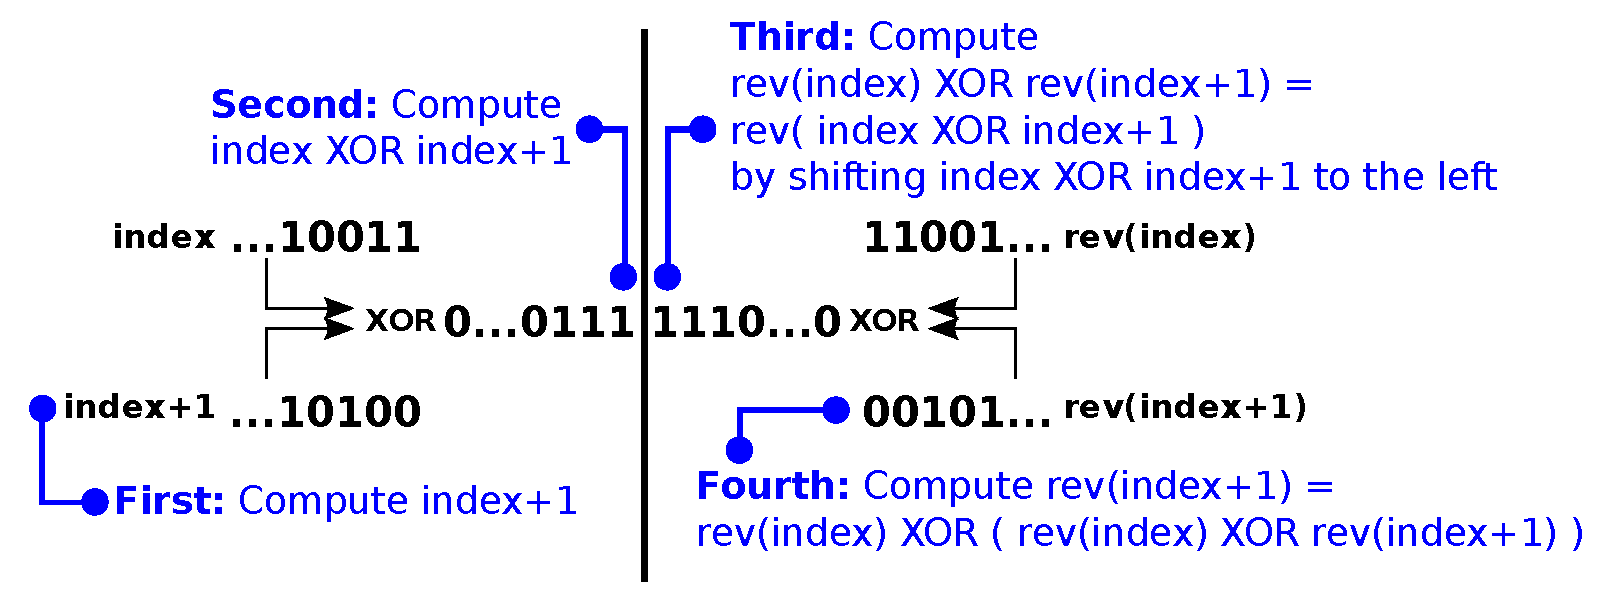
\includegraphics[width=6in]{cartoons/xor.pdf}
\caption{{\bf Bit tersine \c{c}evirme i\c{s}lemi i\c{c}in end\"{u}ktif XOR y\"{o}nteminin 
g\"{o}sterimi.}{\tt index} ile ba\c{s}layarak bit ters de\u{g}eri {\tt rev(index)}, sonraki de\u{g}erler 
({\tt index+1} ve {\tt rev(index+1)}) hesaplan{\i}r. \"{O}nce, {\tt index+1} hesaplan{\i}r. 
Ard{\i}ndan {\tt index} ve {\tt index+1} aras{\i}nda farkl{\i} bitler XOR ile hesaplan{\i}r; 
sonu\c{c}ta elde edilen bit dizgesi {\tt 000\ldots 0111\ldots 1} bi\c{c}imindedir. \"{U}\c{c}\"{u}nc\"{u} olarak,
farkl{\i} bitler {\tt 000\ldots 0111\ldots 1} bi\c{c}iminde olacaklar{\i}ndan, ba\c{s}taki 
s{\i}f{\i}rlar{\i}n say{\i}s{\i}na g\"{o}re bitler kayd{\i}r{\i}l{\i}rarak ters \c{c}evrilebilirler. Son olarak, 
{\tt rev(index+1)} yaln{\i}zca farkl{\i} bitleri \c{c}evirerek (XOR arac{\i}l{\i}\u{g}{\i}yla) hesaplanabilir.
\label{figure:xor}}
\end{figure}

XOR y\"{o}ntemi, bir sonraki dizin ve sonraki ters dizin hesaplamada \c{c}ok etkilidir.
Bununla birlikte, bu hesaplama anl{\i}k olsa bile, algoritma iki nedenden \"{o}t\"{u}r\"{u} vasat bir
performans elde eder: Birinci sebep, ters \c{c}evrilmi\c{s} endekslerin biti\c{s}ik olmayan 
\c{s}ekilde eri\c{s}ilmesidir (dolay{\i}s{\i}yla \"{o}nbellek-optimize edilmemi\c{s}tir). \.{I}kinci sebep, 
{\bf  Listing~\ref{alg:simple-permutation}}'de bulunan {\tt if} ifadesi. Bu {\tt if} ifadesi, 
d\"{o}ng\"{u} a\c{c}{\i}l{\i}m{\i}n{\i}n(derleyici taraf{\i}ndan d\"{o}ng\"{u}n\"{u}n d\"{u}z ak{\i}\c{s}a \c{c}evirilmesi) 
tamamen etkili olmas{\i}n{\i} \"{o}nler, 
\c{c}\"{u}nk\"{u} derleyici \"{o}nceki turda de\u{g}i\c{s}tirilmenin etkilerini bilemeyecektir(bu sorun paralel
olarak takas etme yetene\u{g}ini s{\i}n{\i}rlar). Ayr{\i}ca, d\"{o}ng\"{u} s{\i}ras{\i}nda {\tt index < rev(index)}
frekans{\i} de\u{g}i\c{s}ece\u{g}i i\c{c}in dallanma tahmininin faydalar{\i}n{\i}n azald{\i}\u{g}{\i}na da dikkat edilmelidir.


\paragraph{A\c{c}{\i}lma y\"{o}ntemi (kal{\i}p \"{o}zyinelemeli kapal{\i} form):}

{\tt if (index < rev(index))} kar\c{s}{\i}la\c{s}t{\i}rmas{\i}n{\i} ortadan kald{\i}rmak zordur, \c{c}\"{u}nk\"{u} bunun i\c{c}in
\"{o}nceden hesaplama gerektiren indeksleri hesaplamak ve yaln{\i}zca bu indeksleri ziyaret etmek gerekir.
Bunun do\u{g}ru oldu\u{g}u yerde dizinlerin do\u{g}ru \c{s}ekilde hesaplanmas{\i}, bit tersine \c{c}evirme 
i\c{s}lemine benzerdir. Bununla birlikte, sabit bir boyutta ($b = 10$ bit veya e\c{s}de\u{g}er olarak $n = 1024$)
problemler i\c{c}in, sadece bit-terslenmi\c{s} perm\"{u}tasyon \"{u}zerinden de\u{g}i\c{s}tirilmesi gereken t\"{u}m
indeksleri hesaplamak m\"{u}mk\"{u}nd\"{u}r. Bu, iki a\c{c}{\i}dan yarar sa\u{g}lar. 
Birincisi, d\"{o}ng\"{u}n\"{u}n ba\c{s}{\i}nda, dizinlerde bit tersini ger\c{c}ekle\c{s}tirerek ve {\tt index < rev(index)}'in
tamamen ortadan kald{\i}r{\i}l{\i}p kald{\i}r{\i}lmad{\i}\u{g}{\i}n{\i} kontrol ederek. \.{I}kincisi, derleyici (teorik olarak)
takas i\c{s}lemlerini ard{\i}\c{s}{\i}k olarak biti\c{s}ik olarak yeniden d\"{u}zenleyebilir 
ve b\"{o}ylece \"{o}nbellek performans{\i}n{\i} art{\i}rabilir.

Bu, sabit kodlanm{\i}\c{s} bir i\c{s}lev olan {\tt unrolled\_permutation\_10} ile ger\c{c}ekle\c{s}tirilebilir,
ancak alternatif olarak da derleyici yineleme(template recursion) yoluyla derleme 
zaman{\i}nda bu kodu \"{u}reterek uygulanabilir. {\tt index = z x y} ({\tt z}, {\tt x} ve {\tt y}
biti\c{s}tirilmeleri) bi\c{c}imindeki herhangi bir bit dizesi i\c{c}in 
ters {\tt rev(index) = rev(y) rev(x)   rev(z)} olacakt{\i}r. {\tt z} ve {\tt y} 
bit dizeleri tek bitten olu\c{s}tu\u{g}unda, tersi yok say{\i}labilir: {\tt rev(index) = y   rev(x) z}.
Bu nedenle, her iki u\c{c}tan ba\c{s}lamak (kalan en \"{o}nemli bit ve en az kalan bit kalan) ve
ayn{\i} forma ait problemleri tekrar tekrar olu\c{s}turmak i\c{c}in i\c{c}e do\u{g}ru ilerlemek m\"{u}mk\"{u}nd\"{u}r 
(bu \"{o}zyinelemeli \c{c}a\u{g}r{\i}lar, derleme zaman{\i}nda bunlar{\i} a\c{c}mak i\c{c}in \c{s}ablon \"{o}zyinelemesiyle
uygulanmaktad{\i}r). \c{S}ablon \"{o}zyinelemelerinin bir k{\i}sm{\i} dal{\i}n ve s{\i}n{\i}rlamal{\i} stilde 
({\bf Figure~\ref{figure:unrolled}}) iptal edilebilir, atlanabilir: {\tt index =   1~x~0} bi\c{c}imindeki
bit dizeleri asla {\tt x} bit dizesinin de\u{g}erine bak{\i}lmaks{\i}z{\i}n tersinden daha az olmayacakt{\i}r,
bu nedenle, daha fazla tekrarlama iptal edilebilir. Ayn{\i} \c{s}ekilde, {\tt index = 0~x~1} 
bi\c{c}imindeki bit dizeleri her zaman tersinden daha az olacakt{\i}r ve bu nedenle, 
olas{\i} her {\tt x} i\c{c}in takas i\c{s}lemleri yap{\i}lmal{\i}d{\i}r. Son olarak, {\tt 0~x~0} ve
{\tt 1~x~1} bi\c{c}imlerinin bit dizeleri {\tt x < rev(x)} oldu\u{g}unda terslerinden daha 
az olacakt{\i}r. Bu durumda {\tt index < rev(index)} ancak iki bit daha k\"{u}\c{c}\"{u}k 
oldu\u{g}unda ayn{\i} formda bir sorun olu\c{s}turur ve dolay{\i}s{\i}yla tekrar tekrar y\"{u}r\"{u}t\"{u}lebilir.

Sonu\c{c} olarak, bu y\"{o}ntemin \c{c}al{\i}\c{s}ma zaman{\i}, tekrarlama 
$r(b) = \underbrace{2^{b-2}}_{green} + \underbrace{2 \cdot   r(b-2)}_{yellow} + \underbrace{0}_{red}$ 
({\bf Figure~\ref{figure:unrolled}} i\c{c}indeki renklere kar\c{s}{\i}l{\i}k gelmektedir) ile tan{\i}mlan{\i}r.
$r(1) = 0$ (tek bitle gerekli 0 takas olmas{\i} nedeniyle) ve $r(2) = 1$ (2 bit 
kullanarak bir takas gerekli) kullanarak, bu yineleme $r(b) = 2^{\frac{b}{2}} 
\cdot \left( {(-1)}^b \frac{\sqrt{2}-1}{4} - \frac{1 + \sqrt{2}}{4} \right) + 2^{b-1}$
kapal{\i} formundad{\i}r. Bu nedenle, $b$ \c{c}ift veya tek olup olmad{\i}\u{g}{\i}ndan ba\u{g}{\i}ms{\i}z olarak
$r(b) = 2^{b-1} - c \cdot 2^{\frac{b}{2}}$ ($c=\frac{-1}{2}$, $b$ e\c{s}it oldu\u{g}unda
ve $c=\frac{-1}{\sqrt{2}}$ $b$ tek oldu\u{g}unda). Her hal\"{u}karda, asimtotik \c{c}al{\i}\c{s}ma s\"{u}resi
$2^{b-1}$ teriminin hakimiyeti alt{\i}ndad{\i}r; Bu nedenle, asimptotik \c{c}al{\i}\c{s}ma 
zaman{\i} $n$'in lineer bir fonksiyonudur($n = 2^b$ oldu\u{g}u i\c{c}in).

\begin{figure}
\centering
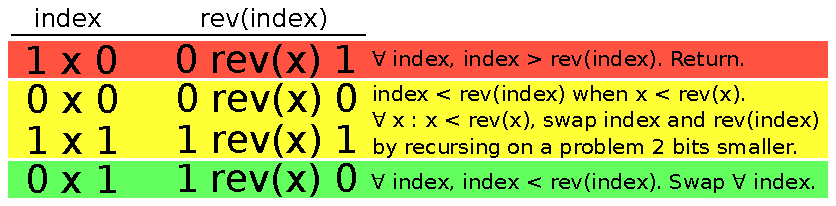
\includegraphics[width=4.5in]{cartoons/unrolled.pdf}
\caption{{\bf Bit tersinmesi i\c{c}in a\c{c}{\i}lm{\i}\c{s} y\"{o}ntemin ill\"{u}strasyonu.}
{\tt index < rev(index)}'in derleme zaman{\i}nda kalan en \"{o}nemli biti ve en az
anlaml{\i} kalan biti ve i\c{c}e do\u{g}ru yinelemeli olarak ilerleyerek bulunmas{\i} olas{\i} 
t\"{u}m bit dizeleri. {\tt 1~x~0} bi\c{c}imindeki bit dizileri hi\c{c}bir zaman tersinden
(k{\i}rm{\i}z{\i} renkle vurgulan{\i}r) daha az olmaz. {\tt 0~x~1} bi\c{c}imindeki bit dizeleri
her zaman tersinden daha az olacakt{\i}r (ye\c{s}il renkle g\"{o}sterilen yer). 
{\tt 0~x~0} ve {\tt 1~x~1} bi\c{c}imlerinin bit dizgileri {\tt x < rev(x)} 
oldu\u{g}unda (sar{\i} renkle g\"{o}sterilen yer) tersi olacakt{\i}r.
  \label{figure:unrolled}}
\end{figure}

K\"{u}\c{c}\"{u}k sorunlar i\c{c}in, bu \c{s}ablon \"{o}zyinelemeli ''a\c{c}{\i}lma'' y\"{o}ntemi \c{c}ok etkilidir.
Bununla birlikte, y\"{o}ntemin bir dezavantaj{\i} b\"{u}y\"{u}k boyutlu problemlerde b\"{u}y\"{u}k 
derleme s\"{u}relerine neden olabilecek ve ayr{\i}ca de\u{g}i\c{s}tirici i\c{s}lemlerin s{\i}ras{\i}n{\i}n
derleyicinin etkili bir \c{s}ekilde optimize edemeyece\u{g}i \c{c}ok say{\i}da kod \"{u}retmesidir.
Asl{\i}nda, ters \c{c}evrilmi\c{s} endekslerin atlanmas{\i} nedeniyle \"{o}nbelle\u{g}i etkili bir 
\c{s}ekilde kullanmak m\"{u}mk\"{u}n olmayabilir. Dolay{\i}s{\i}yla, derleyici ger\c{c}ekle\c{s}tirilen 
takaslar hakk{\i}nda matematiksel bir kavray{\i}\c{s}a sahip olmad{\i}k\c{c}a b\"{u}y\"{u}k boyuttaki problemler 
\"{u}zerindeki a\c{c}{\i}lma y\"{o}nteminin vasat verimlili\u{g}i \"{o}nemli derleme s\"{u}relerini telafi edemez.

\paragraph{\"{O}nbellek ba\u{g}{\i}ms{\i}z \"{o}zyinelemeli bit tersleme perm\"{u}tasyonu:}

$b$ bit say{\i}s{\i} e\c{s}it oldu\u{g}unda dizin dizesi, her biri $\frac{b}{2}$ bitlik 
iki e\c{s}it boyutlu diziye b\"{o}l\"{u}nebilir: {\tt index = x~y}. Ters \c{c}evrilmi\c{s} 
endeks {\tt rev(index)~=~rev(y)~rev(x)} olacakt{\i}r. Bu, \"{u}\c{c} ad{\i}mda hesaplanabilir:
\.{I}lk olarak {\tt x~rev(y)}'yi \"{u}retmek i\c{c}in en d\"{u}\c{s}\"{u}k \"{o}nem derecesini 
({\tt y}'yi olu\c{s}turan) tersine \c{c}evirilir. Ard{\i}ndan, {\tt x} olu\c{s}turan en \"{o}nemli bitleri,
{\tt rev(y)} olu\c{s}turan en az anlaml{\i} bitlerle de\u{g}i\c{s}tirerek {\tt rev(y)~x} \"{u}retilir. 
\"{U}\c{c}\"{u}nc\"{u} olarak, ilk ad{\i}m{\i} yineleyerek ve {\tt rev(y)~rev(x)~=~rev(index)} \"{u}retmek i\c{c}in
en az anlaml{\i} bitler tersine \c{c}evirilir.

Bu \"{o}zyinelemeli teknik yaln{\i}zca ters bir dizin hesaplamak i\c{c}in yararl{\i} de\u{g}ildir:
ayn{\i} zamanda \"{o}nbellek boyutu i\c{c}in ayarlanmaya ihtiya\c{c} duyulmayan lokalize i\c{s}lemlerle
bit ters perm\"{u}tasyonun tekrarlay{\i}c{\i} bir \c{s}ekilde ger\c{c}ekle\c{s}tirilmesi i\c{c}in kullan{\i}labilir.
Birinci ve \"{u}\c{c}\"{u}nc\"{u} ad{\i}mlar birbirine \"{o}zde\c{s} bir \c{s}ekilde uygulan{\i}r: 
olas{\i} t\"{u}m en \"{o}nemli bit dizeleri i\c{c}in, $\frac{b}{2}$ boyutunda daha k\"{u}\c{c}\"{u}k 
yerel bit tersleme perm\"{u}tasyonu ger\c{c}ekle\c{s}tirin. Bu \"{o}zyinelemeli 
bit tersine \c{c}evrilmi\c{s} perm\"{u}tasyonlar{\i}n hepsi daha k\"{u}\c{c}\"{u}k ve biti\c{s}ik bellek bloklar{\i}na
uygulanacak ve b\"{o}ylece \"{o}nbellek performans{\i} artacakt{\i}r. En anlaml{\i} ve en az anlaml{\i}
bit dizelerinin tersine \c{c}evrildi\u{g}i ikinci ad{\i}m, matris transpozisyonuna kar\c{s}{\i}l{\i}k gelir;
en \"{o}nemli bitler matrisin sat{\i}rlar{\i}na ve en az anlaml{\i} bitler s\"{u}tunlara kar\c{s}{\i}l{\i}k gelir
({\tt C}-stili sat{\i}r s\"{u}tun organizasyonu gibi). {\tt x} ve {\tt y} e\c{s}it say{\i}da bit 
kulland{\i}\u{g}{\i}ndan, bu de\u{g}i\c{s}tirme yerinde ger\c{c}ekle\c{s}tirilebilen bir kare matrisinin 
transpozisyonuna kar\c{s}{\i}l{\i}k gelir. Dahas{\i}, matris transpozisyonu i\c{c}in optimal bir
\"{o}nbellek-ba\u{g}{\i}ms{\i}z algoritma (herhangi bir hiyerar\c{s}ik \"{o}nbellek organizasyonu i\c{c}in
m\"{u}mk\"{u}n olan en iyi \c{c}al{\i}\c{s}ma s\"{u}resine eri\c{s}mek anlam{\i}nda)
bilinmektedir ve bu da ilerideki b\"{o}l\"{u}mlere ge\c{c}i\c{s}i ger\c{c}ekle\c{s}tirir\cite{prokop:cache}. 
Dolay{\i}s{\i}yla, bit tersleme perm\"{u}tasyonu, biti\c{s}ik bellek bloklar{\i} de\u{g}i\c{s}imi ve kare matris 
transpozisyonuna indirgenebilir({\bf Figure~\ref{figure:recursive}}).


\begin{figure}
\centering
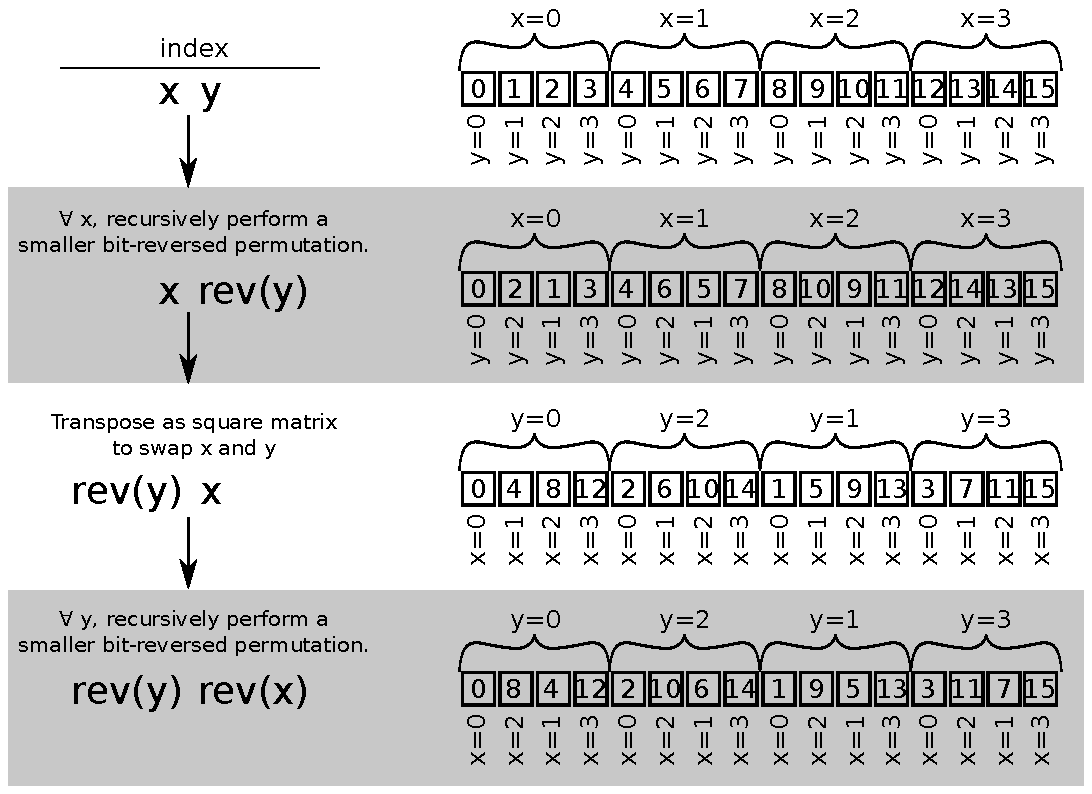
\includegraphics[width=5in]{cartoons/recursive.pdf}
\caption{{\bf Yinelemeli bit tersleme perm\"{u}tasyonunun g\"{o}sterimi.} 
$b$ bit \"{u}zerinde bit terslenmi\c{s} perm\"{u}tasyon, $\frac{b}{2}$ bitte ters \c{c}evrilmi\c{s} s{\i}ralama,
bir kare matrisin yerinde aktar{\i}lmas{\i} ve $\frac{b}{2}$ bitle daha k\"{u}\c{c}\"{u}k bit 
ters perm\"{u}tasyonlar{\i}n ba\c{s}ka bir toplu i\c{s}i olarak ger\c{c}ekle\c{s}tirilir.
Bu ad{\i}mlar{\i}n her birinin mekansal konumu, \"{o}nbellek ba\u{g}{\i}ms{\i}z bir algoritma \"{u}retir.
\label{figure:recursive}}
\end{figure}

$b$ bit say{\i}s{\i} tek oldu\u{g}unda, \"{o}nce tek bir tek-\c{c}ift perm\"{u}tasyonu yap{\i}labilir: 
{\tt index = x~y~z}, {\tt z} tek bitten olu\c{s}an 
{\tt rev(index) = z~rev(y)~rev(x)} d\"{o}nd\"{u}r\"{u}l\"{u}r. Tek-\c{c}ift perm\"{u}tasyon {\tt z~x~y} \"{u}retir.
{\tt z} = 0 iken $b-1$ bit tersine perm\"{u}tasyon ve {\tt z} = 1 oldu\u{g}unda $b-1$ 
bit tersine perm\"{u}tasyon daha uygulayarak {\tt z~rev(y)~rev(x)} elde edilir.
$b$ tek oldu\u{g}unda \"{o}n i\c{s}leme i\c{c}in bu tek-\c{c}ift perm\"{u}tasyon \c{c}al{\i}\c{s}ma s\"{u}resini 
hafif\c{c}e art{\i}racakt{\i}r(bu tek-\c{c}ift perm\"{u}tasyon ayn{\i} zamanda $\frac{n}{2}$ 
boyutundaki bir tampon kullan{\i}larak yerine getirilmektedir).

\"{O}yzinelemenin \c{c}al{\i}\c{s}ma s\"{u}resi $r(b)
= 2 \cdot 2^{\frac{b}{2}} \cdot r(\frac{b}{2}) + 2^b$. Kapal{\i} form olarak
$r(b) = 2^{b-3} \cdot b \cdot c + 2^b \cdot (b-1)$,
burda $c$ sabittir. Sonu\c{c} olarak $r(b) \in \Theta(2^b \cdot b) = \Theta(n
\log(n))$.

$b \gg 1$ oldu\u{g}unda a\c{c}{\i}lm{\i}\c{s} kapal{\i} formdaki kusurlara ra\u{g}men, k\"{u}\c{c}\"{u}k ve
orta b\"{u}y\"{u}kl\"{u}kteki problemler i\c{c}in \c{c}ok etkilidir($b \leq 14$, $n \leq 16384$'ye kar\c{s}{\i}l{\i}k gelir).
Bu nedenle, \"{o}zyinelemeli y\"{o}ntem i\c{c}in ideal bir temel durumdur. 
\"{O}zyinelemeli \c{c}a\u{g}r{\i}lar \c{s}ablon \"{o}zyineleme kullan{\i}larak yap{\i}labilir ve b\"{o}ylece 
derleyici bu \"{o}zyinelemeli \c{c}a\u{g}r{\i}lar taraf{\i}ndan payla\c{s}{\i}lan kodu optimize etmeyi sa\u{g}lar. 
Bu \"{o}zyinelemeli y\"{o}ntem, bit say{\i}s{\i} bir e\c{s}i\u{g}in alt{\i}na d\"{u}\c{s}t\"{u}\u{g}\"{u}nde sadece a\c{c}{\i}lan uygulamay{\i}
\c{c}a\u{g}{\i}rmakla kalmay{\i}p tekrarlama derinli\u{g}i bir e\c{s}i\u{g}i a\c{s}t{\i}\u{g}{\i}nda da a\c{c}{\i}lm{\i}\c{s} uygulamay{\i} 
\c{c}a\u{g}{\i}ran yar{\i} \"{o}zyinelemeli bir y\"{o}ntemi olu\c{s}turur. \c{S}ablon \"{o}zyinelemeli bit tersi 
perm\"{u}tasyonlar{\i}n t\"{u}m\"{u} (daha b\"{u}y\"{u}k tekrarlama derinlikleri i\c{c}in, derleyiciler her 
zaman kodun t\"{u}m sat{\i}rlar{\i}n{\i} a\c{c}amaz; \c{c}\"{u}nk\"{u} bu derleme s{\i}ras{\i}nda \c{c}ok daha y\"{u}ksek 
derleme s\"{u}relerine sebep olabilir, {\tt g++} ve {\tt clang}'da sat{\i}r i\c{c}i
yerle\c{s}tirmeyi zorlayan {\tt attribute~(\_\_always\_inline\_\_)} ile \"{o}zyinelemeli
bit ters perm\"{u}tasyon i\c{s}levi kullan{\i}ld{\i}\u{g}{\i}nda derleyici daha fazla optimizasyona 
izin verebilir). Tek bir \"{o}zyinelemeye izin veren yar{\i} \"{o}zyinelemeli bir y\"{o}ntemin,
$r(\frac{b}{2})$ \"{o}zyinelemeli \c{c}a\u{g}r{\i}lar{\i} kald{\i}r{\i}lan y\"{o}ntemin \c{c}al{\i}\c{s}ma zaman{\i} olan
$2^{\frac{b}{2}}$ ile de\u{g}i\c{s}tirilece\u{g}i i\c{c}in \c{c}al{\i}\c{s}ma zaman{\i} 
$r(b) = 2 \cdot 2^{\frac{b}{2}} \cdot 2^{\frac{b}{2}} + 2^b$'e sahip 
olaca\u{g}{\i}n{\i} unutmay{\i}n. Bu nedenle, yar{\i} \"{o}zyinelemeli y\"{o}ntemin \c{c}al{\i}\c{s}ma 
zaman{\i} $2\cdot 2^b + 2^b \in \Theta(2^b) = \Theta(n)$ olur.

COBRA \"{u}zerinden \"{o}zyinelemeli y\"{o}ntemin bir avantaj{\i} (en az{\i}ndan 
$b$ \c{c}ift oldu\u{g}unda, $\frac{b}{2}$ \c{c}ift oldu\u{g}unda, \ldots taban durum
boyutu veya tekrarlama s{\i}n{\i}r{\i}na ula\c{s}{\i}l{\i}ncaya kadar) tamamen yerinde 
ve bir arabellek olmadan ger\c{c}ekle\c{s}tirilebilir. Yinelemeli y\"{o}ntem, bit 
ters perm\"{u}tasyonun k\"{u}\c{c}\"{u}k ters \c{c}evrilmi\c{s} perm\"{u}tasyonlara 
(her biri ba\u{g}{\i}ms{\i}z ve yerinde bir \c{s}ekilde ger\c{c}ekle\c{s}tirilir) ve 
kare matris transpozisyonuna indirgendi\u{g}inden, SIMD veya GPU'lar \"{u}zerinden yay{\i}n yaparak 
COBRA'n{\i}n paralel hale getirilmesi yar{\i}\c{s} ko\c{s}ullar{\i}n{\i} \"{o}nlemek 
i\c{c}in her bir paralelle\c{s}tirme i\c{c}in yinelenen tamponlar gerektirir.\newline

Asimtotik \c{c}al{\i}\c{s}ma zamanlar{\i} \c{s}u \c{s}ekilde g\"{o}sterilmi\c{s}tir: {\bf
  Table~\ref{table:theoretical-runtimes}}.

\begin{table}[ht!]
  \centering
  \small
  \scalebox{0.88}{
    \begin{tabular}{c|cccccccc}
      & Stockham & Bitwise & Bytewise & Pair bitwise & COBRA & Unrolled & XOR & Recursive \\
      \hline
      %& \multicolumn{3}{c}{$d$ known at compile time} \\
    {\bf Runtime} & \multirow{2}{*}{$n \log(n)$} & \multirow{2}{*}{$n \log(n)$} & \multirow{2}{*}{$n \log(n)$} & \multirow{2}{*}{$n \log(n)$} & \multirow{2}{*}{$n + \frac{n}{t} \log(\frac{n}{t})$} & \multirow{2}{*}{$n$} & $n$ or & $n$ or \\ 
          (asymptotic) & & & & & & & $n \log(\log(n))$ & $n \log(n)$\\
    \hline
    \end{tabular}
  }
  \caption{{\bf Teorik \c{c}al{\i}\c{s}ma zamanlar{\i}.} Her algoritman{\i}n 
  asimtotik \c{c}al{\i}\c{s}ma zamanlar{\i} verilmi\c{s}tir. En d\"{u}\c{s}\"{u}k teorik \c{c}al{\i}\c{s}ma 
  s\"{u}resine sahip algoritmalar{\i}n pratikte \"{u}st\"{u}n 
  olmayabilece\u{g}ini unutmay{\i}n: 
  \"{O}rne\u{g}in, bit-tabanl{\i} ve bayt-tabanl{\i} y\"{o}ntemlerin ikisi de 
  $\in \Theta(n \log(n))$'dir ama bayt-tabanl{\i} y\"{o}ntem bir kerede 8 bit 
  kullanarak s\"{o}zc\"{u}kleri tersine \c{c}evirmek i\c{c}in bir tablo kulland{\i}\u{g}{\i}ndan 
  \"{u}st\"{u}n \c{c}al{\i}\c{s}ma zaman{\i} sabitine sahiptir . Benzer \c{s}ekilde, bit-tabanl{\i}, 
  COBRA ve \"{o}zyinelemeli y\"{o}ntemler daha biti\c{s}ik yerel \c{s}ekillerde 
  belle\u{g}e eri\c{s}ir ve bu nedenle \"{u}st\"{u}n \"{o}nbellek yerle\c{s}imine sahiptir. 
  COBRA y\"{o}ntemi i\c{c}in kullan{\i}lan tampon boyutu $t$'dir. 
  End\"{u}ktif XOR y\"{o}nteminin \c{c}al{\i}\c{s}ma zaman{\i} $\in \Theta(n)$ 
  (ba\c{s}taki s{\i}f{\i}rlar{\i}n say{\i}s{\i} $\Theta(1)$ oldu\u{g}unda) veya 
  $\Theta(n \log(\log(n)))$'t\"{u}r 
  (ba\c{s}taki s{\i}f{\i}rlar{\i}n say{\i}s{\i} donan{\i}mda yap{\i}lamaz ve bu nedenle 
  $\in \Theta(\log(\log(n)))$ ad{\i}m gerektirir). \"{O}zyinelemeli y\"{o}ntem 
  genel olarak $\in \Theta(n \log(n))$ ad{\i}m gerektirir ancak \"{o}zyineleme 
  derinli\u{g}ini s{\i}n{\i}rlayan yar{\i} \"{o}zyinelemeli bir yakla\c{s}{\i}m kullan{\i}ld{\i}\u{g}{\i}nda 
  $\in \Theta(n)$ ad{\i}ma kadar h{\i}zland{\i}r{\i}labilir.}
  \label{table:theoretical-runtimes}
\end{table}

\section*{Sonu\c{c}}
T\"{u}m y\"{o}ntemler {\tt constexpr} de\u{g}i\c{s}kenleri ve i\c{s}levleri ile birlikte
\c{s}ablon \"{o}zyinelemesini kullanan {\tt C++11}'te uygulanm{\i}\c{s}t{\i}r. 
\c{C}al{\i}\c{s}ma zaman{\i} kar\c{s}{\i}la\c{s}t{\i}r{\i}lm{\i}\c{s}, t\"{u}m y\"{o}ntemlerin k{\i}yaslanmas{\i} 
hem {\tt clang++ 3.8.0} hem de {\tt g++ 6.2.0} ile derlenmi\c{s}tir. 
Her iki derleyici de derleme bayraklar{\i} {\tt -Ofast   -march=native -mtune=native} 
ile en iyi duruma getirilmi\c{s}tir. \.{I}\c{s}aret\c{c}i takma ad{\i}n{\i} veya farkl{\i} 
\"{o}l\c{c}\"{u}tler aras{\i}ndaki di\u{g}er etkile\c{s}imi riske sokmamak i\c{c}in, her algoritma 
ve girdi boyutu, ayr{\i} bir {\tt main.cpp} dosyas{\i}nda k{\i}yaslanm{\i}\c{s}t{\i}r. 
{\tt clang++} ile derleme zamanlar{\i} {\bf   Figure~\ref{fig:clang++_compile_times}} 
derleme zamanlar{\i}nda {\bf Figure~\ref{fig:g++_compile_times}} 'de {\tt g++} ile 
\c{c}izilmi\c{s}tir. T\"{u}m y\"{o}ntemler {\tt std::complex<double>} t\"{u}r\"{u}ndeki dizilere uygulanm{\i}\c{s}t{\i}r, 
\c{c}\"{u}nk\"{u} h{\i}zl{\i} bit ters perm\"{u}tasyon ger\c{c}ekle\c{s}tirme konusundaki ana motivasyonumuz 
y\"{o}ntemlerin FFT uygulamas{\i} i\c{c}in uygunlu\u{g}unu de\u{g}erlendirmemizdir. 
Farkl{\i} boyutlardaki ({\tt int} veya {\tt float}) di\u{g}er veri t\"{u}rleri 
kullan{\i}ld{\i}\u{g}{\i}nda, y\"{o}ntemlerin bireysel performanslar{\i}n{\i}n biraz 
de\u{g}i\c{s}ebilece\u{g}ini unutmay{\i}n.

Yerinde ve yerinde olmayan COBRA y\"{o}ntemleri i\c{c}in, her problem boyutu 
i\c{c}in arabellek boyutu optimize edildi. \"{O}nbellek kay{\i}ts{\i}z \"{o}zyinelemeli 
y\"{o}ntem, $b \leq 9$ boyutunda bir taban durumunu kulland{\i}; o boyutta 
bit ters perm\"{u}tasyonun a\c{c}{\i}lmam{\i}\c{s} kapal{\i} formunu hesaplad{\i}. \c{C}al{\i}\c{s}ma zaman{\i}, 
bu taban durumunun boyutu se\c{c}imine kar\c{s}{\i} \c{c}ok hassas de\u{g}ildi; 
bu durum \"{o}nbellek-kay{\i}ts{\i}z matris transpozisyonunda kullan{\i}lan temel durumun 
b\"{u}y\"{u}kl\"{u}\u{g}\"{u}n\"{u} an{\i}msat{\i}r; burada sadece temel durumun hesaplama 
maliyetinin \"{o}nemsiz olmas{\i}n{\i} sa\u{g}layarak \"{o}zyineleme maliyetini 
azaltmak i\c{c}in kullan{\i}l{\i}r.

\"{O}l\c{c}\"{u}len problem boyutlar{\i} $n = 2^8$ (depolamak i\c{c}in $\approx 4$ KB gerektirir) 
ile $n = 2^{30}$ (depolamak i\c{c}in $\approx 16.4$ GB gerektirir) aras{\i}nda 
de\u{g}i\c{s}mektedir. T\"{u}m \"{o}l\c{c}\"{u}mler 100 tekrar ile ortalamas{\i} al{\i}nm{\i}\c{s} ve 
\c{c}al{\i}\c{s}ma zamanlar{\i} \"{o}\u{g}e ba\c{s}{\i}na saniye olarak bildirilmi\c{s}tir (bir bit tersleme 
i\c{c}in ayr{\i}lan s\"{u}re, toplam s\"{u}renin $n$'e b\"{o}l\"{u}m\"{u}). Kar\c{s}{\i}la\c{s}t{\i}rma i\c{c}in 
kullan{\i}lan bilgisayar{\i}n CPU \"{o}zellikleri {\bf Table~\ref{table:cpu_spec}}'de 
listelenmi\c{s}tir. {\tt clang++} ve {\tt g++} ile derlenen t\"{u}m testlerin 
\c{c}al{\i}\c{s}ma zaman{\i} s{\i}ras{\i}yla {\bf Figure~\ref{fig:clang++_runtimes}} ve 
{\bf Figure~\ref{fig:g++_runtimes}} olarak g\"{o}sterilmi\c{s}tir.

Do\u{g}al olarak paralelle\c{s}tirilebilme olan{\i}n{\i} \"{o}l\c{c}mek i\c{c}in, yar{\i} \"{o}zyinelemeli 
y\"{o}ntemin paralel s\"{u}r\"{u}mleri de uygulanm{\i}\c{s} ve kar\c{s}{\i}la\c{s}t{\i}r{\i}lm{\i}\c{s}t{\i}r: Bu \c{c}ok 
\c{c}ekirdekli OpenMP ve {\tt -fopenmp} derleyici se\c{c}ene\u{g}i ile yap{\i}lm{\i}\c{s}t{\i}r. 
Bu OpenMP uygulamas{\i}, paralel olarak \c{c}al{\i}\c{s}t{\i}r{\i}lacak \"{o}zyinelemeli 
\c{c}a\u{g}r{\i}lar{\i}n (sadece bir \"{o}zyinelemeye izin verildi\u{g}i i\c{c}in a\c{c}{\i}lma 
y\"{o}nteminin kapal{\i} form arac{\i}l{\i}\u{g}{\i}yla uygulanmas{\i}na izin vermek i\c{c}in) 
{\tt \#pragma omp parallel for} kullan{\i}r. \.{I}kinci paralel s\"{u}r\"{u}m, CUDA 
arac{\i}l{\i}\u{g}{\i}yla GPU'yu kullanmak i\c{c}in yar{\i} \"{o}zyinelemeli y\"{o}ntemi uyarlar. 
Bu GPU uygulamas{\i}, iki \"{o}zyinelemeye izin verir ve $b=24$ i\c{c}in sabit 
kodlanm{\i}\c{s}t{\i}r (GPU \"{u}zerinden yay{\i}nlanan dizide depolanmas{\i} gereken 
dizinlerin de\u{g}i\c{s}tirilmesini gerektirir). $b=24$ se\c{c}ildi, \c{c}\"{u}nk\"{u} 
$b$ 4'le b\"{o}l\"{u}nebilecek \c{s}ekilde en b\"{u}y\"{u}k problem olarak GPU belle\u{g}ine 
s{\i}\u{g}{\i}yordu(4'le b\"{o}l\"{u}nebilen sorunlar, \"{o}n i\c{s}leme olarak bir 
\c{c}ift-tek perm\"{u}tasyon yapmadan iki tekrarlamayla geni\c{s}letilebiliyordu). 
Bu CUDA uygulamas{\i} ayr{\i}ca GPU'teki yerinde aktar{\i}m{\i} ger\c{c}ekle\c{s}tirir\cite{harris:cuda} 
ve bu nedenle hem \"{o}zyinelemeli aramalar{\i} hem de aktar{\i}m{\i} paralelle\c{s}tirir
(yaln{\i}zca bir kez GPU'ya veri ta\c{s}{\i}mak gibi ek bir avantaja sahiptir). 
Hem OpenMP hem de GPU paralel s\"{u}r\"{u}mleri {\tt clang++}'da s{\i}n{\i}rl{\i} destek 
nedeniyle {\tt g++} (ve GPU s\"{u}r\"{u}m\"{u} {\tt nvcc} kullan{\i}ld{\i}) ile derlendi. 
Bu paralel s\"{u}r\"{u}mler {\bf Figure~\ref{fig:g++_parallel_runtimes}}'te en 
iyi performans g\"{o}steren paralel olmayan y\"{o}ntemlerle kar\c{s}{\i}la\c{s}t{\i}r{\i}lm{\i}\c{s}t{\i}r.

\begin{table}[ht!]
  \centering
  \begin{tabular}{cccccc} L1d &  L1i &    L2 &      L3 & MAX\_SPEED &   RAM \\
\midrule
 32K &  32K &  256K &  15360K &    3.8Ghz &  65GB \\
\end{tabular}
\caption{ {\bf Benchmark i\c{c}in kullan{\i}lan CPU \"{o}zellikleri.} 
L1 veri \"{o}nbellek, L1 y\"{o}nerge \"{o}nbellek, L2 \"{o}nbellek, L3 \"{o}nbellek boyutlar{\i} 
ve saat h{\i}z{\i}n{\i}n yan{\i} s{\i}ra k{\i}yaslama i\c{c}in kullan{\i}lan bilgisayar{\i}n RAM 
boyutu boyutlar{\i} g\"{o}sterilir. Bunu, g\"{o}sterdi\u{g}imiz k{\i}yaslama sonu\c{c}lar{\i}yla 
ili\c{s}kilendirmek i\c{c}in, $32$K $n=2^{11}$, $256$K $n=2^{14}$, 
$15360$K $n=2^{20}$ {\tt std::complex<double>} tipinde
eleman tutabilece\u{g}i farkedilebilir. $65$ GB RAM, $n=2^{31}$ eleman bar{\i}nd{\i}rabilir.
  \label{table:cpu_spec}
}
\end{table}

\begin{figure}[ht!]
\centering
\begin{tabular}{cc}
  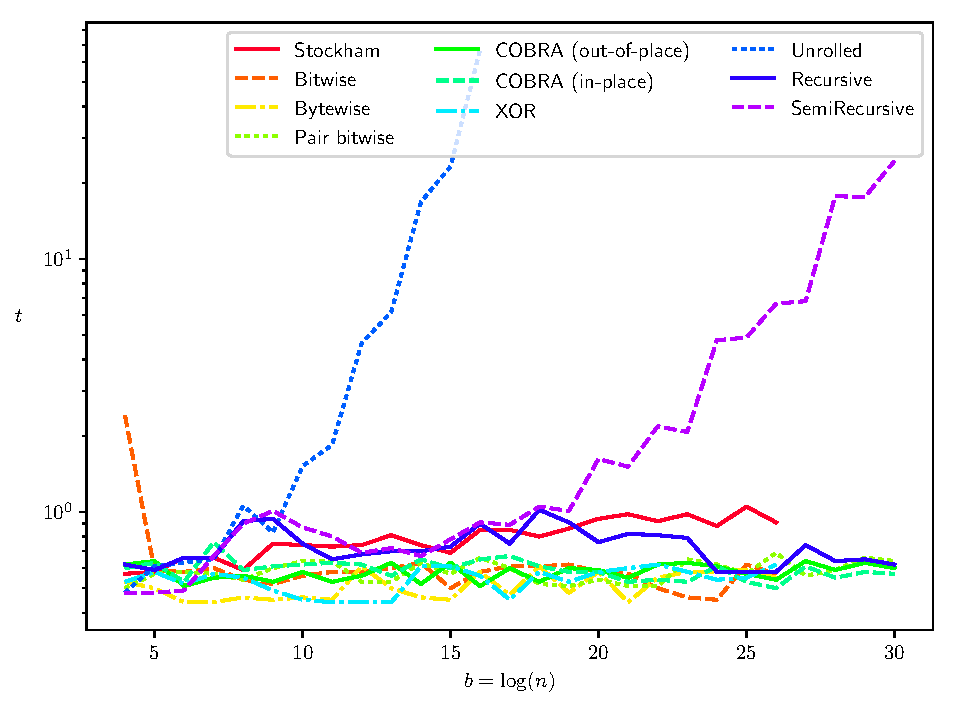
\includegraphics[width=4.5in]{results/clang++_compile_times.pdf}
\end{tabular}
\caption{{\bf {\tt clang++} ile derlenme s\"{u}releri}. 
Her metod i\c{c}in derleme s\"{u}releri g\"{o}sterilmi\c{s}tir. 
$t$-ekseni logaritmik olarak oranlanm{\i}\c{s}t{\i}r. \c{C}al{\i}\c{s}ma s\"{u}releri 
\ref{fig:clang++_runtimes}'de g\"{o}sterilmi\c{s}tir. 
UnrolledShuffle(A\c{c}{\i}lma y\"{o}ntemi) $b>16$ i\c{c}in \c{c}ok 
verimsiz oldu\u{g}undan g\"{o}sterilmemi\c{s}tir.
  \label{fig:clang++_compile_times} 
}
\end{figure}

\begin{figure}[ht!]
\centering
\begin{tabular}{cc}
  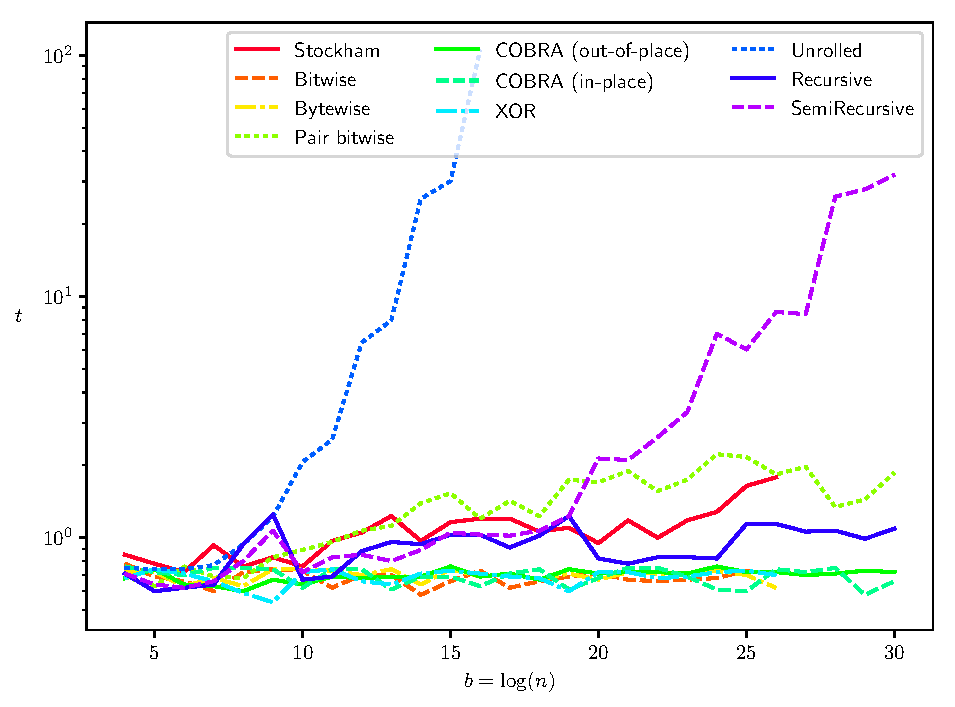
\includegraphics[width=4.5in]{results/g++_compile_times.pdf}
\end{tabular}
\caption{{\bf {\tt g++} ile derlenme s\"{u}releri}.
Her metod i\c{c}in derleme s\"{u}releri g\"{o}sterilmi\c{s}tir. 
$t$-ekseni logaritmik olarak oranlanm{\i}\c{s}t{\i}r. \c{C}al{\i}\c{s}ma s\"{u}releri 
\ref{fig:g++_runtimes}'de g\"{o}sterilmi\c{s}tir. 
UnrolledShuffle(A\c{c}{\i}lma y\"{o}ntemi) $b>16$ i\c{c}in \c{c}ok 
verimsiz oldu\u{g}undan g\"{o}sterilmemi\c{s}tir.
  \label{fig:g++_compile_times} 
}
\end{figure}

\begin{figure}[ht!]
\centering
\begin{tabular}{cc}
  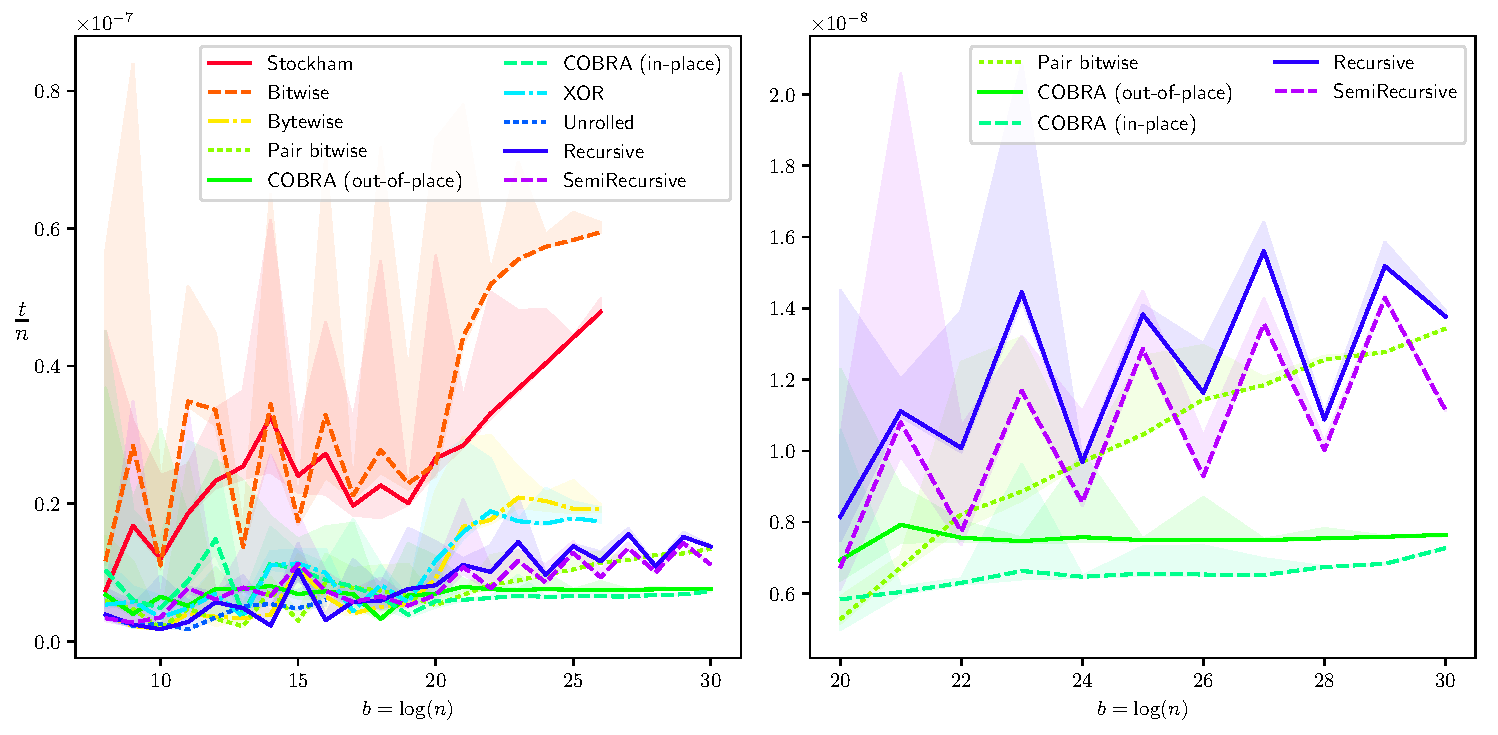
\includegraphics[width=6in]{results/clang++_run_times.pdf}
\end{tabular}
\caption{{\bf {\tt clang++} \c{c}al{\i}\c{s}ma s\"{u}releri}. 
Her y\"{o}ntem i\c{c}in, \c{c}e\c{s}itli boyutlarda bit ters perm\"{u}tasyonlar ger\c{c}ekle\c{s}tirilmi\c{s}tir. 
Her bir y\"{o}ntem ve her problem boyutu i\c{c}in 100 tekrar ile \c{c}al{\i}\c{s}ma 
zaman{\i} (saniye olarak) \"{o}l\c{c}\"{u}lm\"{u}\c{s} ve \"{o}\u{g}e ba\c{s}{\i}na ortalama \c{c}al{\i}\c{s}ma 
s\"{u}resi (ge\c{c}en s\"{u}re $n = 2^b$ ile b\"{o}l\"{u}nm\"{u}\c{s}t\"{u}r) \c{c}izilmi\c{s}tir. 
Her serinin etraf{\i}ndaki g\"{o}lgeli alanlar, 100 kopyan{\i}n tamam{\i}ndaki 
minimum ve maksimum \c{c}al{\i}\c{s}ma s\"{u}relerini g\"{o}stermektedir. Sol panelde, 
$b=4$ - $b=30$ aras{\i}ndaki t\"{u}m y\"{o}ntemler g\"{o}sterilir ve sa\u{g} panel, 
yaln{\i}zca $b=20$ - $b=30$ aras{\i}ndaki daha b\"{u}y\"{u}k sorunlardaki en y\"{u}ksek 
performans serilerini g\"{o}sterir. B\"{u}y\"{u}k sorun ($b>26$) boyutlar{\i}nda d\"{u}\c{s}\"{u}k 
performans g\"{o}steren y\"{o}ntemler (Stockham, bitwise, bytewise ve XOR) 
i\c{c}in kar\c{s}{\i}la\c{s}t{\i}rma d{\i}\c{s}{\i}nda b{\i}rak{\i}lm{\i}\c{s}t{\i}r.
  \label{fig:clang++_runtimes}  
}
\end{figure}

\begin{figure}[ht!]
\centering
\begin{tabular}{cc}
  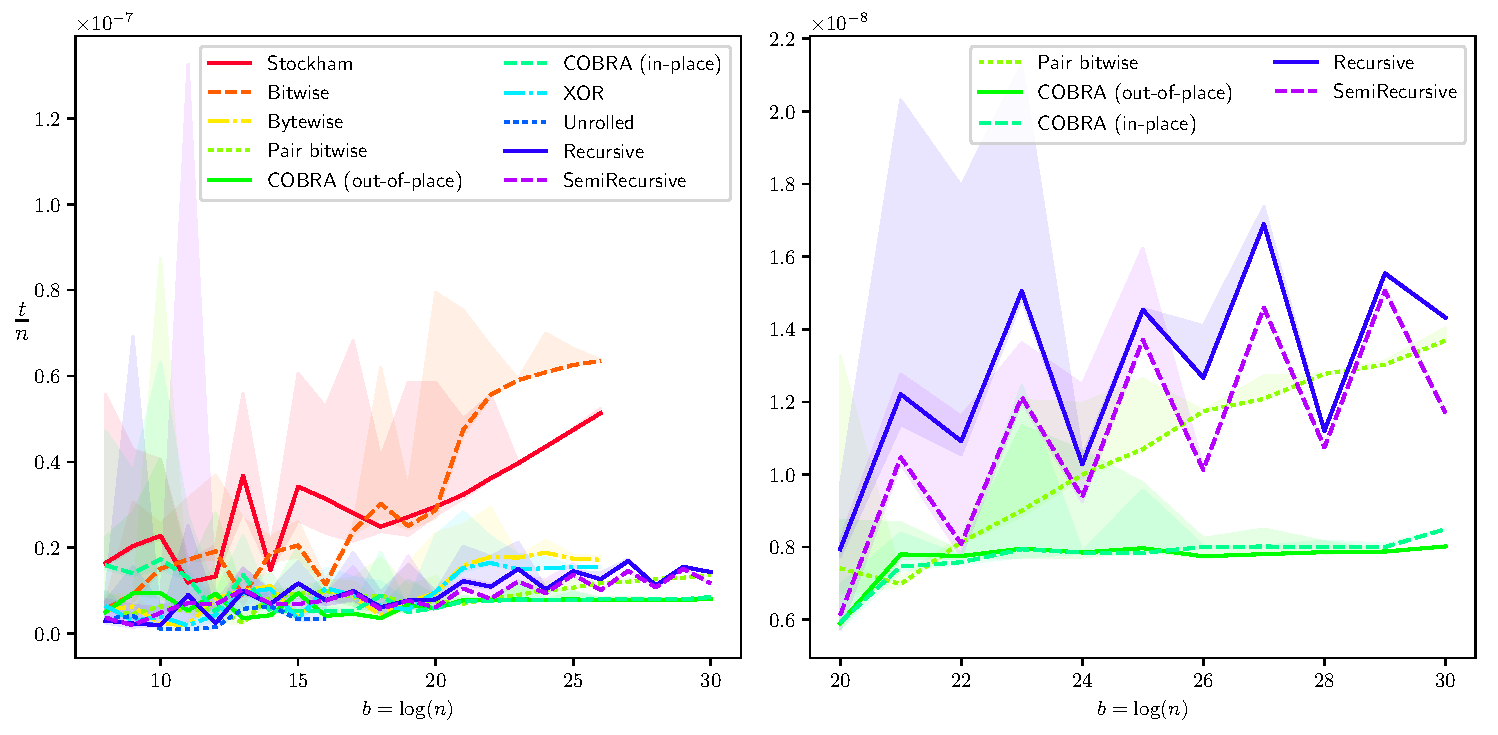
\includegraphics[width=6in]{results/g++_run_times.pdf}
\end{tabular}
\caption{{\bf Eleman ba\c{s}{\i}na {\tt g++} \c{c}al{\i}\c{s}ma s\"{u}releri}. For each method,
Her y\"{o}ntem i\c{c}in, \c{c}e\c{s}itli boyutlarda bit ters perm\"{u}tasyonlar ger\c{c}ekle\c{s}tirilmi\c{s}tir. 
Her bir y\"{o}ntem ve her problem boyutu i\c{c}in 100 tekrar ile \c{c}al{\i}\c{s}ma 
zaman{\i} (saniye olarak) \"{o}l\c{c}\"{u}lm\"{u}\c{s} ve \"{o}\u{g}e ba\c{s}{\i}na ortalama \c{c}al{\i}\c{s}ma 
s\"{u}resi (ge\c{c}en s\"{u}re $n = 2^b$ ile b\"{o}l\"{u}nm\"{u}\c{s}t\"{u}r) \c{c}izilmi\c{s}tir. 
Her serinin etraf{\i}ndaki g\"{o}lgeli alanlar, 100 kopyan{\i}n tamam{\i}ndaki 
minimum ve maksimum \c{c}al{\i}\c{s}ma s\"{u}relerini g\"{o}stermektedir. Sol panelde, 
$b=4$ - $b=30$ aras{\i}ndaki t\"{u}m y\"{o}ntemler g\"{o}sterilir ve sa\u{g} panel, 
yaln{\i}zca $b=20$ - $b=30$ aras{\i}ndaki daha b\"{u}y\"{u}k sorunlardaki en y\"{u}ksek 
performans serilerini g\"{o}sterir. B\"{u}y\"{u}k sorun ($b>26$) boyutlar{\i}nda d\"{u}\c{s}\"{u}k 
performans g\"{o}steren y\"{o}ntemler (Stockham, bitwise, bytewise ve XOR) 
i\c{c}in kar\c{s}{\i}la\c{s}t{\i}rma d{\i}\c{s}{\i}nda b{\i}rak{\i}lm{\i}\c{s}t{\i}r.
  \label{fig:g++_runtimes}  
}
\end{figure}

\begin{figure}[ht!]
\centering
\begin{tabular}{cc}
  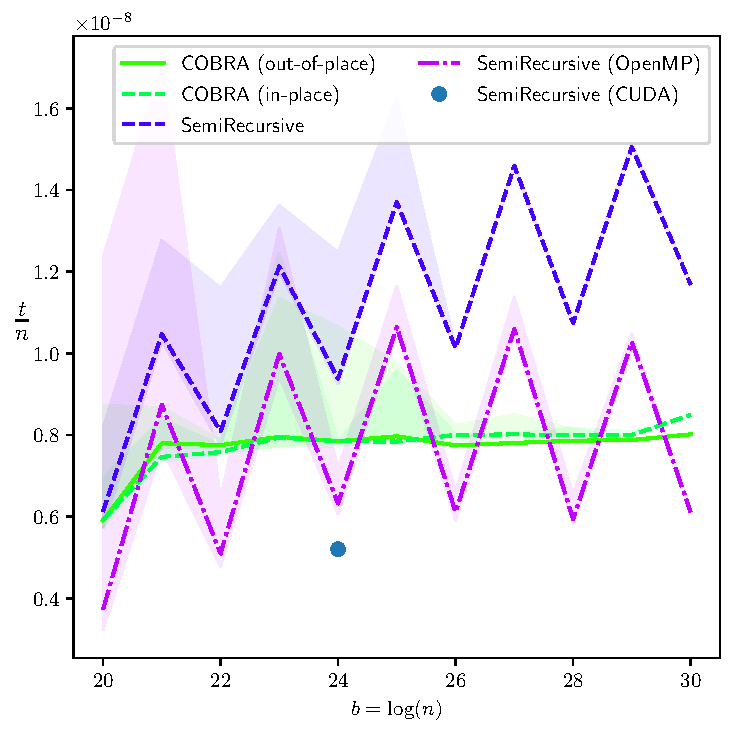
\includegraphics[width=6in]{results/open_mp_performance.pdf}
\end{tabular}
\caption{{\bf Paralelle\c{s}tirmenin performansa olan katk{\i}lar{\i}}.
{\bf Figure~\ref{fig:g++_runtimes}}'in sa\u{g} taraf{\i}ndaki \"{o}l\c{c}\"{u}mler tekrarlanm{\i}\c{s}t{\i}r.
Yar{\i} \"{o}zyineleme metodu paralelle\c{s}tirilerek bu metdolarla k{\i}yaslanm{\i}\c{s}t{\i}r.
Yar{\i} ozyenilemeli metodun yap{\i}s{\i} gere\u{g}i OpenMP ve GPU kullanarak kolayl{\i}kla
paralelle\c{s}tirilmi\c{s}tir ve daha iyi sonu\c{c} vermi\c{s}tir.
  \label{fig:g++_parallel_runtimes}
}
\end{figure}

\section*{Tart{\i}\c{s}ma}

Hem {\tt g++} hem de {\tt clang++} ile, Stockham ve naif bittabanl{\i} 
kar{\i}\c{s}t{\i}rma y\"{o}ntemleri, kabaca birbirlerine benzer bir performansa sahiptir 
ve burada ara\c{s}t{\i}r{\i}lan en az etkili y\"{o}ntemlerdir. Stockham y\"{o}ntemi, yerinde 
olmayan (ekstra bellek kullanan) bir y\"{o}ntemdir (dolay{\i}s{\i}yla \"{o}nbellek 
\"{u}zerindeki y\"{u}k\"{u} artt{\i}r{\i}r) ve bit-tabanl{\i} kar{\i}\c{s}t{\i}rmadan daha fazla 
takas i\c{s}lemi ger\c{c}ekle\c{s}tirir. Bununla birlikte, bitwise y\"{o}ntemi 
verilere daha rasgele bir bi\c{c}imde eri\c{s}irken, Stockham metodu 
\c{c}ift ve tek elemanlara veri eri\c{s}ir ve b\"{o}ylece verilere kabaca 
biti\c{s}ik bir \c{s}ekilde eri\c{s}ir.

Bayt-tabanl{\i} tablo y\"{o}ntemi ve XOR y\"{o}ntemi birbirlerine benzer bir 
performans elde ederler. Her iki y\"{o}ntem de Stockham ve bit-tabanl{\i} 
y\"{o}ntemlerden daha iyi \"{o}l\c{c}eklendirilmi\c{s}tir. Her iki tablo y\"{o}ntemi 
ve XOR y\"{o}ntemi daha h{\i}zl{\i} bit d\"{o}n\"{u}\c{s}\"{u}m\"{u} sa\u{g}lar, ancak biti\c{s}ik bellek 
eri\c{s}im modeli elde edilemez. Dolay{\i}s{\i}yla, ikisinin de \"{o}nbellek 
a\c{c}{\i}s{\i}ndan iyi performans{\i} da yoktur. \"{O}nerilen XOR y\"{o}ntemi  
belle\u{g}in de\u{g}erli oldu\u{g}u sistemlerde (g\"{o}m\"{u}l\"{u} sistemler) 
kullan{\i}labilir, \c{c}\"{u}nk\"{u} $256$B'lik bir tabloyu depolama 
gereksinimi yoktur.

T\"{u}m dizinin L1 \"{o}nbelle\u{g}ine s{\i}\u{g}abilece\u{g}i k\"{u}\c{c}\"{u}k sorunlar i\c{c}in 
d\"{o}ng\"{u}, bit d\"{o}nd\"{u}rme veya dallanma ifadeleri i\c{c}in bir masraf 
olmad{\i}\u{g}{\i} i\c{c}in, a\c{c}{\i}lma yakla\c{s}{\i}m{\i} en iyi performansa ula\c{s}{\i}yor. 
Ayr{\i}ca, i\c{s}lemler derleme kodunda derhal mod adreslemesi 
kullanacak \c{s}ekilde derlenebilir, yani de\u{g}i\c{s}tirilen dizinler 
do\u{g}al olarak derleme komutlar{\i}na kodlan{\i}r ve ayr{\i} bir dizide 
kodlanmaya gerek kalmaz. Bu a\c{c}{\i}lm{\i}\c{s} y\"{o}ntemin \c{c}al{\i}\c{s}ma zaman{\i} 
faydas{\i}, daha b\"{u}y\"{u}k sorunlara (dizi L1 veya L2 \"{o}nbelleklerine 
s{\i}\u{g}mad{\i}\u{g}{\i} i\c{c}in) uzanmaz ve a\c{c}{\i}lmam{\i}\c{s} y\"{o}ntemin derleme 
zaman{\i} \c{c}ok pahal{\i} olur (yakla\c{s}{\i}k 100 saniye, $b=16$ ile 
{\tt g++} ve {\tt clang++} i\c{c}in ).

B\"{u}y\"{u}k problemler \"{u}zerinde en performansl{\i} algoritmalar, 
\"{o}nbellek ak{\i}lda bulundurularak tasarlanm{\i}\c{s} algoritmalard{\i}r: 
Bu bit-tabanl{\i} \c{c}ift y\"{o}ntemini, COBRA y\"{o}ntemini 
(yerinde ve yerinde olmayan) ve \"{o}zyinelemeli y\"{o}ntemi ve 
yar{\i} \"{o}zyinelemeli versiyonunu i\c{c}erir. Yinelemeli ve yar{\i} 
\"{o}zyinelemeli y\"{o}ntemler, \c{c}ift say{\i}daki bitlere i\c{c}eren 
problemlerin uygulanmas{\i}nda faydal{\i} olur \c{c}\"{u}nk\"{u} bir 
\"{o}n i\c{s}leme basama\u{g}{\i} olarak \c{c}ift-tek perm\"{u}tasyonuna ihtiya\c{c} 
duyulmaz (bu olay b\"{u}y\"{u}k problemlerin \c{c}al{\i}\c{s}ma zamanlar{\i}nda 
testere di\c{s}i deseniyle sonu\c{c}lan{\i}r). Yar{\i} \"{o}zyinelemeli 
y\"{o}ntem \"{o}zyinelemeli y\"{o}ntemden biraz daha y\"{u}ksek bir 
performans sa\u{g}lar, ancak bunu derleme s\"{u}resinin uzat{\i}lmas{\i} pahas{\i}na sa\u{g}lar
($b=28$ ile {\tt g++} ve {\tt clang++} kullan{\i}ld{\i}\u{g}{\i}nda 
10 ila 13 saniye aras{\i}nda bir farkla). Daha k\"{u}\c{c}\"{u}k sorunlar 
i\c{c}in, yerinde olmayan COBRA y\"{o}ntemi, \"{o}nbellekte iki kat 
daha fazla bellek kullanman{\i}n y\"{u}k\"{u} daha b\"{u}y\"{u}k oldu\u{g}undan, 
yerinde olan versiyonundan daha az verimlidir. Bununla 
birlikte daha b\"{u}y\"{u}k sorunlar i\c{c}in yerinde olmayan COBRA 
y\"{o}ntemi ile daha y\"{u}ksek bir performans elde edilir; 
\c{c}\"{u}nk\"{u} yerinde bir y\"{o}ntem de\u{g}erleri arabellek arac{\i}l{\i}\u{g}{\i}yla de\u{g}i\c{s}tirir,
yerinde olmayan y\"{o}ntem ise de\u{g}erleri fazladan bir bellek 
yoluyla kopyalar.

Bit \c{c}ifti tersi y\"{o}ntemi daha fazla takas i\c{s}lemi ger\c{c}ekle\c{s}tirir, 
ancak daha b\"{u}y\"{u}k yerellik ve bir sonu\c{c} tamponu kullan{\i}lmadan 
(Stockham gibi yerinde olmayan algoritmalar taraf{\i}ndan gerekli 
oldu\u{g}unun aksine). \c{C}ifti bitwise y\"{o}ntemi, COBRA y\"{o}ntemi, \"{o}zyinelemeli 
ve yar{\i} \"{o}zyinelemeli y\"{o}ntemler b\"{u}y\"{u}k problemler i\c{c}in kabaca benzer 
\c{s}ekilde \c{c}al{\i}\c{s}{\i}r. Yerinde olmayan COBRA y\"{o}ntemi daha b\"{u}y\"{u}k 
sorunlar i\c{c}in biraz daha iyi performans g\"{o}sterir, ancak i\c{s}lemci 
kazan\c{c}lar{\i} CPU i\c{c}in matris arabellek boyutu optimize edilmedi\u{g}inde 
s\"{o}n\"{u}kt\"{u}r. \"{O}nbellek s{\i}n{\i}rlar{\i}ndaki durumlarda \"{o}\u{g}eler ba\c{s}{\i}na \c{c}al{\i}\c{s}ma 
zaman{\i}nda k\"{u}\c{c}\"{u}k art{\i}\c{s}lar vard{\i}r, \"{o}zellikle yerinde y\"{o}ntemler 
i\c{c}in $b=18$'de ve yerinde olmayan y\"{o}ntemler i\c{c}in $b=17$'de 
kar\c{s}{\i}la\c{s}{\i}lan L3 \"{o}nbellek s{\i}n{\i}r{\i}nda bu g\"{o}r\"{u}lebilir.

Bir matris tamponu arac{\i}l{\i}\u{g}{\i}yla i\c{s}leyen COBRA y\"{o}ntemlerinden 
farkl{\i} olarak, \"{o}zyinelemeli ve yar{\i} \"{o}zyinelemeli y\"{o}ntemler 
do\u{g}al olarak \"{o}nbellek verimli olur ve b\"{o}yle bir arabellek kullanmaz. 
Bu nedenle paralellik i\c{c}in \c{c}ok uygundurlar. 
{\bf Figure~\ref{fig:g++_parallel_runtimes}} fig\"{u}r\"{u}, OpenMP ile 
paralellik ekleyerek veya GPU ile paralellik ekleyerek 
ger\c{c}ekle\c{s}tirilebilecek g\"{u}\c{c}l\"{u} performans avantaj{\i}n{\i} g\"{o}sterir. 
\"{O}zyinelemelerin di\u{g}er \"{o}\u{g}elerden gelen herhangi bir bilgiye eri\c{s}mesi 
gerekmedi\u{g}inden paralellik i\c{c}in m\"{u}kemmeldir. Yinelemeli ve 
yar{\i} \"{o}zyinelemeli y\"{o}ntemlere \"{o}zg\"{u} bu paralelle\c{s}tirilebilir 
nitelik, GPU kodunu daha da optimize edilerek daha b\"{u}y\"{u}k 
bir etkiye sahip olabilir.

{\bf Figure~\ref{fig:g++_parallel_runtimes}}'te g\"{o}sterildi\u{g}i gibi 
$b=24$'de, paralel olmayan en h{\i}zl{\i} y\"{o}ntemin \c{c}al{\i}\c{s}ma zaman{\i}, 
\"{o}\u{g}e ba\c{s}{\i}na $8 \times {10}^{-9}$ saniyenin alt{\i}nda veya 
toplamda yakla\c{s}{\i}k $0.13$ saniye gerektirir. Buna kar\c{s}{\i}l{\i}k, 
yar{\i} \"{o}zyinelemeli y\"{o}ntemin OpenMP varyant{\i} kabaca $0.1$ saniye 
gerektirir ve yar{\i} \"{o}zyinelemeli y\"{o}ntemin GPU varyant{\i} $0.08$ saniye 
gerektirir. Bir referans noktas{\i} olarak, {\tt numpy} FFT 
({\tt FFTPACK} library'si kullan{\i}r) bu boyuttaki sorunlar i\c{c}in 
kabaca 2 saniye s\"{u}rmektedir. Saf bit yakla\c{s}{\i}m{\i}, toplam FFT 
\c{c}al{\i}\c{s}ma s\"{u}resinin yakla\c{s}{\i}k \%50'sini bit tersine perm\"{u}tasyonda 
harcanaca\u{g}{\i}ndan bu k{\i}s{\i}m kabaca 1 saniyeye ihtiya\c{c} duyuyor; 
yani bu daha h{\i}zl{\i} bit ters perm\"{u}tasyon y\"{o}ntemlerini 
kullanman{\i}n h{\i}zlanmas{\i}n{\i}n \"{o}nemsiz oldu\u{g}u anlam{\i}na geliyor. 
FFT kelebek kodu karma\c{s}{\i}k say{\i}lar{\i}n daha karma\c{s}{\i}k manip\"{u}lasyonlar{\i}n{\i} 
ger\c{c}ekle\c{s}tirmesine ra\u{g}men, bit ters perm\"{u}tasyonu 
g\"{o}r\"{u}nd\"{u}\u{g}\"{u}nden daha \"{o}nemli hale getirerek tamamen biti\c{s}ik bir 
bi\c{c}imde bunu yapar. Ayr{\i}ca, t\"{u}m i\c{s}lemi GPU \"{u}zerinde yapmak 
paralel olarak k\"{u}\c{c}\"{u}k FFT 
kelebek i\c{s}lemlerini paralelle\c{s}tirmenin yan{\i}nda, 
verileri kopyalaman{\i}n maliyetinden ka\c{c}{\i}narak, 
bit tersine \c{c}evirmenin \c{c}al{\i}\c{s}ma s\"{u}resini b\"{u}y\"{u}k \"{o}l\c{c}\"{u}de azaltacakt{\i}r.

\"{O}zyinelemeli y\"{o}ntemler paralelle\c{s}tirme yetene\u{g}inin yan{\i} s{\i}ra, 
belirli bir \"{o}nbellek mimarisi i\c{c}in ayar yapmadan y\"{u}ksek performans 
elde etmeleriyle de avantajl{\i}d{\i}rlar(bu \"{o}nbellek sorunu 
COBRA y\"{o}ntemlerinin verimlili\u{g}ini \"{o}nemli derecede etkilemektedir). 
\"{O}zyinelemeli y\"{o}ntem \"{o}nbellek-kay{\i}ts{\i}zd{\i}r ve matris transpozisyonu 
i\c{c}in en uygun \"{o}nbellek kay{\i}ts{\i}z y\"{o}ntemi\cite{prokop:cache} ile e\c{s}le\c{s}tirildi\u{g}inde, 
\"{o}nbellek mimarisi hakk{\i}nda bilgi sahibi olmadan olduk\c{c}a 
biti\c{s}ik bellek eri\c{s}imlerini garanti eder. Yinelemeli y\"{o}ntemde oldu\u{g}u gibi, 
yar{\i} \"{o}zyinelemeli strateji de \"{o}nbellek performans{\i} i\c{c}in ayarlanma 
ihtiyac{\i} duymaz. Bununla birlikte, yar{\i} \"{o}zyinelemeli y\"{o}ntem 
\"{o}nbellek-kay{\i}ts{\i}z de\u{g}ildir, \c{c}\"{u}nk\"{u} b\"{u}y\"{u}k problemler, yine de \"{o}nbelle\u{g}e 
s{\i}\u{g}mayan daha k\"{u}\c{c}\"{u}k bit-tersine perm\"{u}tasyon problemlerine indirgenebilir. 
\"{O}zyinelemeli y\"{o}ntem, paralelle\c{s}tirmeden elde edilen performans 
avantaj{\i}n{\i} ara\c{s}t{\i}ran gelecekteki ara\c{s}t{\i}rmalar i\c{c}in sadece ilgin\c{c} 
olmakla kalmaz, ayr{\i}ca mimariye \"{o}zg\"{u} \"{o}nbellek ayar{\i} yap{\i}lmadan 
y\"{u}ksek performans elde etmesi, en uygun \"{o}nbellek-bilinmeyen 
y\"{o}ntemi geli\c{s}tirmek i\c{c}in umut verici bir dayanak noktas{\i}d{\i}r.

\section*{Ula\c{s}{\i}labilirlik}
T\"{u}m {\tt C++11} kaynak kodlar{\i}, GPU algoritmas{\i}n{\i}n kodlar{\i}, 
kullan{\i}lan scriptler ve makalenin \LaTeX\ versiyonu eri\c{s}ime a\c{c}{\i}kt{\i}r
(Creative Commons license alt{\i}nda) ve
\url{https://bitbucket.org/orserang/bit-reversal-methods} adresinden eri\c{s}ilebilir.\newline

\section*{Te\c{s}ekk\"{u}rler}

Thimo Wellner ve Guy Ling katk{\i}lar{\i}ndan dolay{\i} te\c{s}ekk\"{u}r ederiz.\newline 

\noindent 
Bu makale Freie Universit\"at Berlin'de 2016--2017 
k{\i}\c{s} e\u{g}itim d\"{o}neminde Oliver Serang
taraf{\i}ndan verilen bir dersin par\c{c}as{\i} olarak yaz{\i}lm{\i}\c{s}t{\i}r.
Makalenin \c{c}al{\i}\c{s}an \"{o}\u{g}rencilerin dilindeki \c{c}evirilerine (Almanca, \c{C}ince, \.{I}spanyolca)
repository i\c{c}indeki linklerden ula\c{s}{\i}labilir. Bu versiyon esas versiyon de\u{g}ildir.
%fixme: add these links after the translations are finished

\section*{Yazar Katk{\i}lar{\i}}
Yeni algoritmalar ve paralel olmayan implementasyonlar 
proje y\"{o}neticisi O.S. taraf{\i}ndan yap{\i}lm{\i}\c{s}t{\i}r. Giri\c{s} b\"{o}l\"{u}m\"{u} X.W.
taraf{\i}ndan yaz{\i}lm{\i}\c{s}t{\i}r. Metodlar k{\i}sm{\i} ve \c{c}al{\i}\c{s}ma s\"{u}releri incelemeri
B.A., X.W., ve D.W. taraf{\i}ndan yap{\i}lm{\i}\c{s}t{\i}r. OpenMP k{\i}s{\i}mlar{\i} O.S. GPU
k{\i}s{\i}mlar{\i} B.A. taraf{\i}ndan geli\c{s}tirilmi\c{s}tir. \"{O}l\c{c}\"{u}mler, fig\"{u}rler ve sonu\c{c} 
b\"{o}l\"{u}m\"{u} C.K. taraf{\i}ndan yap{\i}lm{\i}\c{s}t{\i}r. Tart{\i}\c{s}ma b\"{o}l\"{u}m\"{u} X.W. ve O.S. taraf{\i}ndan
haz{\i}rlanm{\i}\c{s}t{\i}r. Testler ve optimizasyonlar B.A. ve D.W., son \"{o}l\c{c}\"{u}mler 
C.K., L.I., T.C., ve O.S. taraf{\i}ndan yap{\i}lm{\i}\c{s}t{\i}r.\newline

% at end of this section:
\noindent O.S. ve T.C. haricindeki yazar s{\i}ralamas{\i} \"{o}\u{g}renciler taraf{\i}ndan
gizli oylamayla belirlenmi\c{s}tir.

% bibliography:
\bibliographystyle{unsrt}
\bibliography{refs}


\end{document}

